\chapter{Equip Expectation Maximization with Normalizing Flows}
\label{chpt6:em-flow}
\graphicspath{{source/chapter6/}}

When learning with partially observed variables in graphical models, EM is one of the most widely used frameworks in practices. In directed graphical models, immediate relief is that we do not need to deal with the partition function $Z(\bm{\theta})$ anymore. However, it does not mean directed graphical models with partially observed variables are trivial to learn. The 'missing' data (corresponding to unobserved variables) still poses challenges in model learning, since we want to have the partial evidence (observed) well explained by our model while keeping its ability to track uncertainty of the 'unobserved' part.

As discussed in section~\ref{chpt2:sec:learning-principles}, the presence of latent or hidden variables is either due to the data availability or abstraction of data generating. Once the dataset is given, the option left to us is the choice of the model that we plan to use to approximate the true distribution $p^{\ast}$ which actually generated the dataset. This process is to select one model from a set of models, i.e. hypothesis space, based on the likelihood criteria. If the hypothesis space is very limited, the ability to represent our true $p^{\ast}$ is limited, leading to the inherent error. This type of inherent limitation brings learning \textit{bias} before we start to fit the parameters.
Therefore, given that the dataset is large and representative enough, we hope that the hypothesis space is highly expressive such that we are more likely to be able to represent $p^{\ast}$ with a selected model from the hypothesis space. This naturally requires our model to be flexible and expressive.

Gaussian mixture model has been successfully applied widely with EM framework, which also enjoys the closed-form update rule in iterations. The advantage comes with the limitation of linear dependency and free parameters that can be tuned, i.e. limitation of flexibility. To explore further, we discuss more flexible models beyond Gaussian in this chapter. We start by inducing the normalizing flows that are going to be used as probabilistic models in place of Gaussian models. A normalizing flow can consist of as many non-linear transformations as needed, and thus is highly flexible. Besides, likelihood computation ability remains and it allows efficient sampling in normalizing flow. But closed-form iterative update solutions are not available anymore. We, therefore, need to design the practical algorithms to model learning in EM framework.


\section{Normalizing Flow}
\label{chpt6:sec:flow}
Normalizing flow is a practical approach to improve the flexibility of probabilistic models while still keeping the likelihood computation tractable and the efficiency of generating samples. The general idea is to start with an initial random variable following a relatively simple distribution with known probability density function. Then a chain of invertible parameterized transformations is applied to the initial random variable such that the output follows a more flexible distribution.

Denote the chain of transformations by $\tilde{\bm{g}}$ and the output by $\tilde{\bm{x}}\in \RR^{N}$. Then we have
\begin{equation}
  \tilde{\bm{x}}=\tilde{\bm{g}}(\bm{z})
\end{equation}
where $\bm{z}\in \RR^{N}$ is the initial random variable with know density function $p(\bm{z})$. To explicitly denote the chain,
\begin{equation}
  \tilde{\bm{g}}=\tilde{\bm{g}}^{[L]}\circ \tilde{\bm{g}}^{[L-1]}\circ \cdots
  \circ \tilde{\bm{g}}^{[1]},
\end{equation}
which is invertible $\tilde{\bm{f}}=\tilde{\bm{g}}^{-1}$. Then the signal flow can be depicted as% , illustrated in \autoref{illustation}.
\begin{equation*}
  \centering
  \begin{tikzpicture}
    \node (z) at (0,0) {};
    \node at ($(z)-(0.5,0)$){$\bm{z}=\bm{h}_0$};
    \node (xi1) at (1.5,0) {$\bm{h}_1$};
    \node (xi2) at (3,0) {};
    \node (xi3) at (4.5,0){};
    \node (x) at (6,0) {};
    \node at ($(x)+(0.5,0)$){$\tilde{\bm{x}} = \bm{h}_L$};
    \draw[->] ($(z) + (0.3,0.1)$) -- node[above]{$\tilde{\bm{g}}^{[1]}$} ($(xi1)+(-0.3,0.1)$); 
    \draw[->] ($(xi1)-(0.3,0.1)$) -- node[below]{$\tilde{\bm{f}}^{[1]}$}($(z) - (-0.3,0.1)$);
    \draw[->] ($(xi1) + (0.3,0.1)$) -- node[above]{$\tilde{\bm{g}}^{[2]}$} ($(xi2)+(-0.3,0.1)$); 
    \draw[->] ($(xi2)-(0.3,0.1)$) -- node[below]{$\tilde{\bm{f}}^{[2]}$}($(xi1) - (-0.3,0.1)$);
    \draw[->] ($(xi3) + (0.3,0.1)$) -- node[above]{$\tilde{\bm{g}}^{[L]}$} ($(x)+(-0.3,0.1)$); 
    \draw[->] ($(x)-(0.3,0.1)$) -- node[below]{$\tilde{\bm{f}}^{[L]}$}($(xi3) - (-0.3,0.1)$);
    \draw[dotted,line width = 0.3 mm] (xi2) -- (xi3);
  \end{tikzpicture}
\end{equation*}
where $\tilde{\bm{g}}^{[l]}$ and $\tilde{\bm{f}}^{[l]}$ are the $l$-th transformation in $\tilde{\bm{g}}$ and $\tilde{\bm{f}}$, respectively. In practice, $\bm{\tilde}{g}$ can be implemented by feed-forward neural networks, which we will detail later.

If every transformation in the chain of the flow is invertible, the full mapping is invertible.
Then, the probability density function relation between $p(\bm{z})$ and $p(\tilde{\bm{x}})$ follows the change of variable formula
\begin{equation}\label{chpt6:eq:change-var}
  p(\tilde{\bm{x}}) =  p(\bm{z}) \bigg| \mathrm{det}(\bm{J}) \big|_{\bm{z}=\tilde{\bm{f}}(\tilde{\bm{x}})}\bigg|,
\end{equation}
where $\mathrm{det}(\bm{J})$ denotes the determinant of Jacobian $\bm{J}$
\begin{equation}
  \bm{J} = \left[
    \begin{array}{ccc}
      \frac{\partial \tilde{f}_1}{\partial \tilde{x}_1} & \hdots & \frac{\partial \tilde{f}_1}{\partial \tilde{x}_N} \\
      \vdots & \hdots & \vdots \\
      \frac{\partial \tilde{f}_N}{\partial \tilde{x}_1} & \hdots & \frac{\partial \tilde{f}_N}{\partial \tilde{x}_N}
    \end{array}
  \right].
\end{equation}
The challenge lies at the determinant computation of Jacobian $\bm{J}$, or equivalently that of each transformation $\tilde{\bm{g}}^{[l]}$. \cite{DBLP:journals/corr/DinhKB14} introduced the model NICE to transform only half of the variables at a chain step, which results in triangular Jacobian of the transformation. If each transformation has a triangular Jacobian, determinant computation would be efficient in \eqref{chpt6:eq:change-var}.
This flow architecture divides the feature $\bm{h}_l$ at the $l$'th layer into two subparts as
$\bm{h}_l = [\bm{h}_{l,a}^{\intercal} \, , \, \bm{h}_{l,b}^{\intercal}]^{\intercal}$ where
$(\cdot)^{\intercal}$ denotes transpose operation. We have the following forward and inverse relations between $(l-1)$'th and $l$'th layers:
\begin{align}\label{eq-gl}
  \bm{h}_{l-1} &=
                 \begin{bmatrix}
                   \bm{h}_{l-1,a}\\
                   \bm{h}_{l-1,b}
                 \end{bmatrix}
  =
  \begin{bmatrix}
    \bm{h}_{l,a}\\
    \bm{m}_a(\bm{h}_{l,a})\odot \bm{h}_{l,b} + \bm{m}_b(\bm{h}_{l,a})
  \end{bmatrix},\nonumber\\
  \bm{h}_{l} &=
               \begin{bmatrix}
                 \bm{h}_{l,a}\\
                 \bm{h}_{l,b}
               \end{bmatrix}
  =
  \begin{bmatrix}
    \bm{h}_{l-1,a}\\
    \left(  \bm{h}_{l-1,b} - \bm{m}_b(\bm{h}_{l-1,a}) \right)\oslash \bm{m}_a(\bm{h}_{l-1,a}) 
  \end{bmatrix}, 
\end{align}
where $\odot$ denotes element-wise product, $\oslash$ denotes
element-wise division, and $\bm{m}_a(\cdot), \bm{m}_b(\cdot)$ can be
complex non-linear mappings (implemented by neural networks).
For the flow model, the determinant of Jacobian matrix is
\begin{equation}
  \mathrm{det}(\bm{J}) |_{\bm{z}=\tilde{\bm{f}}(\tilde{\bm{x}})} = \prod_{l=1}^L \det (\bm{J}_l) |_{\bm{h}_{l}},
\end{equation}
where $\bm{J}_l$ is the Jacobian of the transformation from the $l$-th layer to the $(l-1)$-th layer, i.e., the inverse transformation. We compute the determinate of the Jacobian matrix as
\begin{align}\label{eq-hl-determinate}
  \det (\bm{J}_l)|_{\bm{h}_{l}}& = \det \left[  \pd{\bm{h}_{l-1}}{\bm{h}_l} \right] \nonumber\\
                               & = \det
                                 \begin{bmatrix}
                                   \bm{I}_a & \mathbf{0} \nonumber\\
                                   \pd{\bm{h}_{l-1,b}}{\bm{h}_{l,a}} & \mathrm{diag}(\bm{m}_a(\bm{h}_{l,a}))
                                 \end{bmatrix}\nonumber\\
                               &= \det \left( \mathrm{diag}(\bm{m}_a(\bm{h}_{l,a})) \right),
\end{align}
where $\bm{I}_a$ is identity matrix and $\mathrm{diag}(\cdot)$ returns a square matrix with the elements of $(\cdot)$ on the main diagnal. Then the probability density function of $\tilde{\bm{x}}$ is
\begin{align}
  p(\tilde{\bm{x}}) & =  p(\bm{z}) \big| \mathrm{det}(\bm{J}) |_{\bm{z}=\tilde{\bm{f}}(\tilde{\bm{x}})}\big| \nonumber\\
                    &  = p(\bm{z}) \prod_{l=1}^L \abs{\det\left( \mathrm{diag}(\bm{m}_a(\bm{h}_{l,a}))  \right)}.
\end{align}

\eqref{eq-gl} describes a \textit{coupling} mapping between layers. Since the coupling has a partial identity mapping, direct concatenation of multiple such coupling mappings would result in a partial identity mapping of the overall mapping $\tilde{\bm{g}}$. Therefore, techniques such as alternating the positions of identity mapping \cite{2016arXiv160508803D} or using $1\times1$ convolution operations \cite{2018arXiv180703039K} before each coupling mapping are used to treat the issue.
Sometimes, it may not be necessary to carry all features thorough all $L$ chain steps. For instance, \cite{2016arXiv160508803D}\cite{2018arXiv180703039K} split some hidden
layer signal $\bm{h}$ and model a part of it directly as standard Gaussian to reduce computation and memory burden.

\begin{remark}
  There are alternative ways of formulating the transformation of variable changing. A popular one is the Inverse autoregreeesive flow (IAF) proposed in \cite{rezende2015variational}. In the IAF model, a chain step of transformation is formulated as
  \begin{equation*}
    \bm{h}_l = \bm{h}_{l-1} + \bm{u} \cdot {m}(\bm{w}^{\intercal} \cdot \bm{h}_{l-1} + b)
  \end{equation*}
  where $m$ is non-linear mapping, $\bm{w}, \bm{u}~\in \RR^{N}$ and $b\in \RR$. IAF does no use partial identity mapping as NICE. Its Jacobian is not triangular and thus determinant computation is more expensive. Moreover, whether it is invertible depends on the mapping $m$. The followed work by \cite{kingma2016IVF} created element-wise transformation in a customized way to improve IAF such its Jacobian and inverse are easier to compute. 
  
  In contrast to the above finite-chain flow where $L$ is a discrete finite integer, the method developed in \cite{ricky2018ODE} introduced a continuous-transformation of variables by solving an ordinary differential equation (ODE). Comparing to the discrete finite chain of transformation in normalizing flow, ODE can be viewed as a continuous chain of variable transformation. The inverse mapping and Jacobian determinant are not required in ODE method. But ODE needs to solve differentiation equations which is also challenging.
\end{remark}

\section{Generator mixture model and EM training}

\begin{figure}[tp!]
  \centering
  \begin{tikzpicture}
    % \tikzstyle{enode} = [thick, draw=blue, circle, inner sep = 3pt,
    % align=center]
    \tikzstyle{enode} = [thick, draw=black, circle, align=center]
    \tikzstyle{cnode} = [thick, draw=black, circle, align=center, inner sep = 0.3pt]
    
    \tikzstyle{nnode} = [thick, rectangle, rounded corners = 2pt,minimum size = 0.8cm,draw,inner sep = 12pt]
    \node[enode] (z) at (-1.5,2) {$\bm{z}$};
    \node[enode] (x) at (0,0){$\bm{x}$};
    \node[enode] (s) at (0,2){$\bm{s}$};
    \node[nnode, fit=(x)(z)(s)] (box) {};
    % \node[] at (-1.8,-0.4) {$\abs{\Dd}$};

    \node[enode] (pi) at (1.5,2){$\bm{\pi}$};
    \node[cnode] (phi) at (1.5,0){$\{ \bm{\theta}_k \}$};
    
    \draw[->] (z) to (x);
    \draw[->] (s) to (x);
    \draw[->] (pi) to (s);
    \draw[->] (phi) to (x);

  \end{tikzpicture}
  \caption{Graphical Model of GenMM.}\label{chpt6:fig:genmm-graph}
\end{figure}

\begin{figure}[tp!]
  \centering
  \begin{tikzpicture}
    \tikzstyle{enode} = [thick, draw=black, ellipse, inner sep = 2pt,  align=center]
    \tikzstyle{nnode} = [thick, rectangle, rounded corners = 2pt,minimum size = 0.8cm,draw,inner sep = 2pt]
    \node[enode] (z) at (0,0) {$\bm{z}\sim p(\bm{z})$};
    \node[enode] (x) at (5.5,0){$\bm{x}\sim p(\bm{x}; \bm{\Theta})$};
    % \node at (5.2,-1) {$p(\bm{x};\bm{\Phi}) = \textstyle\sum_{k=1}^K \pi_k  p_k(\bm{x})$};
    \node[nnode] (g1) at (2.6,1.8) {$\bm{g}_1$};
    \node[nnode] (g2) at (2.6,0.5) {$\bm{g}_2$};
    \node[nnode] (gk) at (2.6,-1.8) {$\bm{g}_K$};
    \draw[dotted,line width=2pt] (2.6,-0.3) -- (2.6,-1.2);
    \draw[->] (z) [in= 180, out =0] to (g1);
    \draw[->] (z) [in= 180, out =0] to (g2);
    \draw[->] (z) [in= 180, out =0] to (gk);
    \filldraw[->] (3.7, 0.5)circle (2pt) -- node[above=0.2]{$\bm{s}\sim \bm{\pi}$} (x) ;
    % \draw[->] (3,-0.8) -- (3.5, -0.8);
    \draw[->] (g1) -- (3.5,1.8);
    \draw[->] (g2) -- (3.5, 0.5);
    \draw[->] (gk) -- (3.5, -1.8);
  \end{tikzpicture}
  \caption{Signal diagram of GenMM.}\label{dia-emgm-nm}
\end{figure}

In this section, we introduce a generative model that is a mixture of $K$ flow models. All the $K$ flow models have a common input latent variable $\bm{z} \in \mathbb{R}^N$. Here, a flow $\bm{g}_k(\bm{z}): \mathbb{R}^N
\rightarrow \mathbb{R}^N$ is a instance of $\tilde{\bm{g}}$. $\bm{g}_k$ acts as the $k$-th generator and depends on a set of parameters $\bm{\theta}_k$ as
$\bm{g}_k(\bm{z})=\bm{g}(\bm{z};\boldsymbol{\theta}_k)$. For
simplicity, we assume that all $K$ generators have the same
chain structure. Furthermore, the distribution of $\bm{z}$ is fixed as Gaussian $\mathsf{N}(\bm{0},\bm{I})$.
The induced probability density function of $\bm{x} \in \mathbb{R}^N$ of the proposed mixture model with $K$ mixture components is given as:
\begin{align}\label{eq:FirstMixtureModel}
  p(\bm{x};\bm{\Theta})  &= \textstyle\sum_{k=1}^K \pi_k  p_k(\bm{x}) \nonumber\\
                         &= \textstyle \sum_{k=1}^K \pi_k  p(\bm{g}_k(\bm{z}))\nonumber\\
                         &= \textstyle \sum_{k=1}^K \pi_k  p(\bm{g}(\bm{z};\boldsymbol{\theta}_k)).
\end{align}
We use $\bm{\Theta}$ to denote the set of all parameters $ \{\bm{\pi},\bm{\theta}_1, \dots, \bm{\theta}_K \}$, where $\bm{\pi} = \left\{ \pi_1, \hdots, \pi_K \right\}$ is the prior distribution of the generators. Note that $\pi_k \geq 0$ and $\sum_{k=1}^K \pi_k =1$. The mixture model
in \eqref{eq:FirstMixtureModel} is called a generator mixture model (GenMM). The graphical model of GenMM is illustrated in Figure~\ref{chpt6:fig:genmm-graph}. The plate in this figure is common notation in template models (see \cite[section~6]{koller2009pgm}), denoting we can instantiate multiple tuple $(\bm{z}, \bm{x}, \bm{s})$ instances having dependency as illustrated. Furthermore, the
signal diagram of GenMM is illustrated in Figure~\ref{dia-emgm-nm}. The GenMM can be considered as a high-complexity model because each mixture component $p_k(\bm{x})$ has its own parameter set $\bm{\theta}_k$. 
% the parameter $\boldsymbol{\theta}_k$ varies across $K$ mixture components.

The maximum likelihood estimation problem is
\begin{equation}\label{eq:max-genmm}
  \hat{\bm{\Theta}} = \uargmax{\bm{\Theta}}{\log{\prod_{\bm{x}^{i} \in \Dd} p(\bm{x}^{i};\bm{\Theta})}},
\end{equation}
where the superscript $i$ corresponds to the $i$'th data sample in a given dataset.
We address the above maximum likelihood estimation problem using EM. 
Let us use a categorical variable $\bm{s} = [s_1, s_2, \cdots, s_K]$
for $1$-of-$K$ representation to be a hidden variable that indicates which generator is the actual one. Elements of $\bm{s}$ follow $s_k \in \{0,1\}$, $\sum_{k=1}^K s_k =1$, and $p(s_k=1)=\pi_k$. The variable $\bm{s}$ is the hidden variable in EM. We will use $\gamma_k$ to denote the posterior probability $p(s_k =1|\bm{x})$ calculated as
\begin{align}\label{eq-genmm-gamma}
  \gamma_k = p(s_k =1|\bm{x};\bm{\Theta}) 
  = \frac{\pi_k p(\bm{g}(\bm{z};\bm{\theta}_k))}{\sum_{l=1}^K\; \pi_l p(\bm{g}(\bm{z};\bm{\theta}_l))}.
\end{align}
Assume that a value $\bm{\Theta}^{\mathrm{old}}$ of the parameter set $\bm{\Theta}$ is given, the iterative steps in EM algorithm update $\bm{\Theta}$ as follows.
\begin{enumerate}
\item E-step: Evaluation of $\gamma_{k}^{i}$ is 
  \begin{equation}\label{eq-genmm-e-step}
    \gamma_{k}^{i}(\bm{\Theta}^{\mathrm{old}}) = \frac{\pi_k^\mathrm{{old}} p(\bm{g}(\bm{z}^{i};\bm{\theta}_k^{\mathrm{old}}))}{\sum_{l=1}^K\; \pi_l^\mathrm{{old}} p(\bm{g}(\bm{z}^{i};\bm{\theta}_l^{\mathrm{old}}))}.   
  \end{equation}
\item M-step: Evaluation of $\bm{\Theta}^{\mathrm{new}}$ given by
  \begin{equation}\label{eq-genmm-opt}
    \bm{\Theta}^{\mathrm{new}} =   \uargmax{\bm{\Theta}}{\mathcal{Q} (\bm{\Theta},\bm{\Theta}^{\mathrm{old}})}, 
  \end{equation}
  where the expected likelihood is
  \begin{equation}
    \hspace{-8pt}\mathcal{Q} (\bm{\Theta},\bm{\Theta}^{\mathrm{old}}) = \sum_{i}\sum_{k} \gamma_{k}^{i}(\bm{\Theta}^{\mathrm{old}}) \log \pi_k p_k(\bm{x}^{i}).
  \end{equation}
\end{enumerate}

For the GenMM in \eqref{eq:FirstMixtureModel}, realizing EM requires computation of $\gamma_k$ in the E-step and computation of the joint likelihood $\log{\pi_k p_k(\bm{x})}$ in the M-step. They require explicit computation of the conditional density $p_k(\bm{x}) =  p(\bm{g}_k(\bm{z})) =p(\bm{g}(\bm{z};\bm{\theta}_k))$. This is fulfilled by flow realization of generator $\bm{g}_k$. Since the chain-step transformations can be any complex mapping as discussed in section~\ref{chpt6:sec:flow}, they can be implemented by neural networks. The neural network implementation allows high flexibility of GenMM in representing complex-structured multi-modal data.

\subsubsection{EM Learning of GenMM}
\label{sec-algo-genmm}
The mixture model GenMM is illustrated in Figure~\ref{dia-emgm-nm},
where $K$ generators with a certain prior distribution share the same
latent distribution $p(\bm{z})$. With a neural network based flow as the generator $\bm{g}_k$ for the $k$'th mixture component in GenMM, the probability density function $p_k(\bm{x})$ for any
$\bm{x}$ can be computed exactly. Recall that $p_k(\bm{x}) =  p(\bm{g}_k(\bm{z})) =p(\bm{g}(\bm{z};\bm{\theta}_k))$ and let $\bm{f}_k$ be the inverse of $\bm{g}_k$. Then, the posterior probability can be computed further from \eqref{eq-genmm-e-step} as
\begin{align}\label{eq-genmm-gamma}
  \gamma_k({\bm{\Theta}}^{\mathrm{old}}) = \frac{\pi_k^{\mathrm{old}} p(\bm{f}_k(\bm{x})) \big|\det\left( \pd{\bm{f}_k(\bm{x})}{\bm{x}} \right)\big|}{\sum_{j=1}^K\; \pi_j^{\mathrm{old}} p(\bm{f}_j(\bm{x})) \big|\det\left( \pd{\bm{f}_j(\bm{x})}{\bm{x}} \right)\big|},
\end{align}
and the objective function in the M-step can be written as
\begin{align}\label{eq-genmm-obj}
  &\Qq\left(\bm{\Theta},\bm{\Theta}^{\mathrm{old}}\right)  \nonumber\\
  =&\sum_{i=1}^{\abs{\Dd}} \sum_{k=1}^{K}\gamma_k^{(i)}(\bm{\Theta}^{\mathrm{old}})\bigg[ \log\;\pi_k +\log\;p(\bm{f}_k(\bm{x}^{(i)})) + \log\;\bigg|\det\left(\pd{\bm{f}_k(\bm{x}^{(i)})}{\bm{x}^{(i)}} \right)\bigg|\bigg].
\end{align}
We usually deal with a large dataset for model learning, i.e. $\abs{\Dd}$ can be large. In that case we implement the EM algorithm in batch fashion. 
Recall that $ \bm{\Theta}= \{\bm{\pi},\bm{\theta}_1, \dots, \bm{\theta}_K \}$ and hence the M-step optimization problem $\argmax_{\bm{\Theta}} \mathcal{Q} (\bm{\Theta},\bm{\Theta}^{\mathrm{old}})$ is addressed in two steps:
\begin{itemize}
\item[(a)] optimizing w.r.t. $\{ \bm{\theta}_k \}_{k=1}^{K}$,
\item[(b)] optimizing w.r.t. $\bm{\pi}$.
\end{itemize}

Finding a closed-form solution for the problem $\argmax{\{\bm{\theta}_k\}_{k=1}^{K}}{ \mathcal{Q} (\bm{\Theta},\bm{\Theta}^{\mathrm{old}})}$ is not feasible in general. Instead, we do the batch-size gradient decent to optimize w.r.t. $\{\bm{\theta}_k\}_{k=1}^{K}$.
Further, optimization in the batch fashion leads to a practical problem as follows. 
Since $\bm{\theta}_k$ is the parameter set of neural networks $\bm{g}_k$, one update step of gradient decent would update the generator $\bm{g}_k$ and we would lose the old mixture model parameter set $\bm{\Theta}^{\mathrm{old}}$ that is needed to compute the posteriors $\gamma_k(\bm{\Theta}^{\mathrm{old}})$ and to update $\bm{\pi}$. Thus, in learning GenMM, we maintain two such models with parameter sets $\bm{\Theta}$ and $\bm{\Theta}^{\mathrm{old}}$, respectively. At the beginning of an EM step, $\bm{\Theta} = \bm{\Theta}^{\mathrm{old}}$. While we optimize $\{\bm{\theta}_k\}_{k=1}^{K}$ of $\bm{\Theta}$ with batch-size gradient decent, we use the model with old parameter set $\bm{\Theta}^{\mathrm{old}}$ to do posterior computation and update of $\bm{\pi}$. At the end of the EM step, the old parameter set is replaced by the updated one: $\bm{\Theta}^{\mathrm{old}}\gets \bm{\Theta}$.


\begin{algorithm}[t]
  \caption{EM for learning GenMM}\label{flow-algo-em}
  \begin{algorithmic}[1]
    \STATE {\bfseries Input:}
    Latent distribution: $p(\bm{z})$. Empirical distribution $P_d(\bm{x})$ of the input dataset;
    \STATE Set a total number of epochs $T$ for training, a prior distribution $\bm{\pi}$, EM update gap $t_{\mathrm{EM}}$;
    \STATE  Set a learning rate $\eta$. 
    \STATE Build two models with parameter sets:
    \STATE ${\bm{\Theta}}^{\mathrm{old}}=\{ \bm{\pi}^{\mathrm{old}},
    \bm{\th}_1^{\mathrm{old}},\hdots,
    \bm{\th}_K^{\mathrm{old}} \}$,
    \STATE ${\bm{\Theta}} = \{ \bm{\pi},
    \bm{\th}_1,\hdots, \bm{\th}_K \}$.
    \STATE Initialize the generator prior distribution $\pi_k = 1/K$;\\ Initialize $\bm{\theta}_k$ of $\bm{g}_k$, for all $k=1,\dots,K$ randomly. 
    \STATE $\bm{\Theta}^{\mathrm{old}} \gets \bm{\Theta}$.
    \FOR { {epoch} $t < T$}
    \FOR{the iteration in epoch $t$} %\Comment{M-Step}
    \STATE Sample a batch of data $\left\{ \bm{x}^{(i)}
    \right\}_{i=1}^{n_b}$ from the dataset $\Dd$ 
    \STATE Compute $\gamma_k^{i}(\bm{\Theta}^{\mathrm{old}})$ as in \eqref{eq-genmm-gamma},
    for all $\bm{x}^{i}$ and $k=1, \dots, K$
    % \Comment{Calculate posterior \autoref{eq-posterior-gamma}}
    \STATE Compute
    $\Qq\left(\bm{\Theta},\bm{\Theta}^{\mathrm{old}}\right)$ as in \eqref{eq-genmm-obj}%\Comment{Expectation}
    
    \STATE $\partial{g_k} \gets \nabla_{\bm{\th}_k} \frac{1}{n^{b}}\Qq\left(
      \bm{\Theta}, \bm{\Theta}^{\mathrm{old}}\right)$,
    $\forall \bm{\th}_k \in \bm{\Theta}$
    \STATE $\bm{\th}_k \gets \bm{\th}_k + \eta \cdot \partial{g_k}$, $\forall \bm{\th}_k \in \bm{\Theta}$
    \ENDFOR
    % \STATE $\th_k^{t+1} \gets \th_k$, $\forall k$ %\Comment{Update new
    % parameters}
    \IF{$(t \mod t_{\mathrm{EM}} ) = 0$}
    \STATE $\pi_k \gets \EE_{\Dd}\left[ \gamma_k \right]$ %\Comment{Update perior}
    \STATE $\bm{\Theta}^{\mathrm{old}} \gets \bm{\Theta}$.
    \ENDIF
    \ENDFOR
  \end{algorithmic}
\end{algorithm}

Then we discuss the optimization of the prior distribution $\bm{\pi}$. The optimization problem is 
\begin{equation}\label{eq-pi-update1}
  \bm{\pi}^{\mathrm{new}} = \uargmax{\bm{\pi}}{ \mathcal{Q}
    (\bm{\Theta},\bm{\Theta}^{\mathrm{old}})}, \,\,
  \mathrm{s.t.} \sum_{k=1}^{K}\pi_k = 1.
\end{equation}
The update of prior follows the solution
\begin{equation}\label{eq-pi-solution}
  \pi_k^{\mathrm{new}} = \frac{1}{\abs{\Dd}}\sum_{i=1}^{\abs{\Dd}}\gamma_k^{i}(\bm{\Theta}^{\mathrm{old}}).
\end{equation}
The detail to get the solution is derived in the section~\ref{subsubsec:Proof_for_update}. For a given dataset with empirical distribution $P_d(\bm{x})$,
$\gamma_k$ is evaluated with batch data in order to calculate the cost
$\Qq\left(\bm{\Theta},\bm{\Theta}^{\mathrm{old}}\right)$ and to update the
parameter $\bm{\theta}_k$ of $\bm{g}_k$. We accumulate the values of $\gamma_k$ of batches and
average out for one epoch to update $\bm{\pi}$, {i.e.}, $\pi_k \gets \EE_{\Dd}\left[ \gamma_k \right]$.



We summarize the EM algorithm for GenMM in Algorithm~\autoref{flow-algo-em}.
In implementation, to avoid numerical computation problem, $\log{p(\bm{g}(\bm{z}; \bm{\theta}_k))}$ is
scaled by the dimension of signal $\bm{x}$ in order to compute $\gamma_k$. 

\subsubsection{Details for Update of $\pi$}
\label{subsubsec:Proof_for_update}

The optimization of $\bm{\pi}$ is addressed in the following Lagrangian form
\begin{equation}
  \Ff(\bm{\Theta}) = \mathcal{Q}(\bm{\Theta},\bm{\Theta}^{\mathrm{old}}) + \lambda
  \left( 1 - \sum_{k=1}^{K}\pi_k \right),
\end{equation}
where $\lambda$ is the Lagrange multiplier. Then
\begin{align}
  \bm{\pi}^{\mathrm{new}} =& \uargmax{\bm{\pi}}{ \Ff(\bm{\Theta})} \nonumber\\
  =&  \uargmax{\bm{\pi}}{}\sum_{i=1}^{\abs{\Dd}}
     \sum_{k=1}^{K}\gamma_k^{i}(\bm{\Theta}^{\mathrm{old}})\bigg[
     \log\;\pi_k +   \log\;p(\bm{f}_k(\bm{x}^{i})) \nonumber \\
                           &+ \log\;\bigg|\det\left(
                             \pd{\bm{f}_k(\bm{x}^{i})}{\bm{x}^{i}}
                             \right)\bigg|\bigg] + \lambda  \left( 1 - \sum_{k=1}^{K}\pi_k \right) \nonumber\\
  =& \uargmax{\bm{\pi}}{} \sum_{i=1}^{\Dd}
     \sum_{k=1}^{K}\gamma_k^{i}(\bm{\Theta}^{\mathrm{old}})
     \log\;\pi_k+ \lambda  \left( 1 - \sum_{k=1}^{K}\pi_k \right),
\end{align}
where $\bm{f}_k = \bm{g}_k^{-1}$. Then solving
\begin{equation}
  \pd{\Ff}{\pi_k} = 0, k=1, 2, \cdots, K,
\end{equation}
we get 
$
\pi_k = \frac{1}{\lambda}
\sum_{i=1}^{n}\gamma_k^{i}(\bm{\Theta}^{\mathrm{old}}), \forall k.
$
With condition $\sum_{k=1}^{K}\pi_k =1$, we have
$
\lambda = \sum_{k=1}^{K}\sum_{i=1}^{\abs{\Dd}}\gamma_k^{i}(\bm{\Theta}^{\mathrm{old}}) =\abs{\Dd}.
$
Therefore, the solution is
$
\pi_k = \frac{1}{\abs{\Dd}}
\sum_{i=1}^{\abs{\Dd}}\gamma_k^{i}(\bm{\Theta}^{\mathrm{old}}), \forall k.
$
Note that the updated prior parameter $\pi_k$
is non-negative due to the non-negativity of the posterior $\gamma_k^{i}$.

\subsection{On Convergence of GenMM}
Now we analysis the convergence behaviour of GenMM. Under some conditions, GenMM converges. In what follows we present the convergence arguments.

\begin{proposition}
  Assume that for all $k$, the parameters $\bm{\theta}_k$ are in a compact set such that the corresponding mapping $\bm{g}_k$ is invertible. Assume further that all generator mappings fulfill that $\bm{f}_k$ and $\frac{\partial \bm{f}_k}{\partial \bm{x}}$ are continuous functions of $\bm{\theta}_k$. Then GenMM converges. 
  % Suppose that all the generator mappings $\bm{g}_k$ are such that $\bm{f}_k$ and $\frac{\partial \bm{f}_k}{\partial \bm{x}}$ are continuous functions of $\bm{\theta}_k$. Assume further that for all $k$, the parameters $\bm{\theta}_k$ are in a compact set such that the corresponding mapping $\bm{g}_k$ is invertible. Then GenMM converges. 
  % \textcolor{red}{Do you think it is possible to say: The GenMM converges to a saddle point. In that case the confusion about usual understanding on convergence to local minima does not arise.}
\end{proposition}
\begin{proof}
  Assume that the assumption holds. Then the determinant term $\det(\bm{J})$ in \eqref{chpt6:eq:change-var} is a continuous function of $\bm{\theta}_k$. Due to \eqref{chpt6:eq:change-var} and the continuity of Gaussian density $p(\bm{z})$, the probability density function $p_k(\bm{x})$ is a continuous function of $\bm{\theta}_k$. Therefore, $p(\bm{x})$ given in \eqref{eq:FirstMixtureModel} is a continuous function of $\bm{\Theta}$. Denote the likelihood in \eqref{eq:max-genmm} as $\Ll(\bm{\Theta})=\log \textstyle\prod_{i} p(\bm{x}^{(i)};\bm{\Theta})$. The maximum value of $\Ll(\bm{\Theta})$ is bounded due to continuity of $p(\bm{x})$ w.r.t. $\bm{\Theta}$.
  Define $\hat{F}(\bm{\Theta}) = \Qq\left(\bm{\Theta},\bm{\Theta}^{\mathrm{old}}\right) - \sum_{i=1}^{\abs{\Dd}}\sum_{k=1}^{K}\gamma_k^{i}(\bm{\Theta}^{\mathrm{old}}) \log\gamma_k^{(i)}(\bm{\Theta}^{\mathrm{old}})$ (note $\hat{F}$ is the empirical version of lower bound in \eqref{chpt5:eq:lower-bound-F}). It is well known that $\hat{F}(\bm{\Theta})$ is a lower bound on the likelihood function $\Ll(\bm{\Theta})$, i.e. $\Ll(\bm{\Theta}) \geq \hat{F}(\bm{\Theta})$. Note that the essence of EM algorithm is that the likelihood function value is elevated by increasing the value of its lower bound $\hat{F}(\bm{\Theta})$. Since the maximum value of the log-likelihood $\Ll(\bm{\Theta})$ is finite, $\hat{F}(\bm{\Theta})$ can not grow unbounded.
  % Actually the maximization of $\Ll(\bm{\Phi})$ solved by EM is done by keeping increasing a lower bound of likelihood $\Ll(\bm{\Phi})$: 
  % .
  % The inequality  always holds.
  % $\mathcal{Q}(\cdot,\bm{\Phi}^{\mathrm{old}})$ can not grow unbounded, i.e., the EM converges under the %assumption as $\mathcal{Q}(\bm{\Phi}^{\mathrm{new}},\bm{\Phi}^{\mathrm{new}})\geq %\mathcal{Q}(\bm{\Phi}^{\mathrm{old}},\bm{\Phi}^{\mathrm{old}})$ after each iteration.

  % \textcolor{red}{Therefore an important issue is that the log-likelihood is finite. But, is there any chance that it can not hold? Means somehow it goes unbounded. What is the condition that likelihhod function is guaranteed to be finite with its parameters?}
\end{proof}


\section{A low-complexity model}
There are $K$ flow generators implemented as neural networks in GenMM, which makes GenMM a high-complexity model.
We now propose a low-complexity model where parameters are shared. This is motivated by many machine learning setups where model parameters are shared across model components. For example, this techniques is applied as use of shared covariance matrices in a tied Gaussian mixture model, in linear discriminant analysis \cite{bellegarda1990tiedmixture, Kimball:1993:UTD:1075671.1075694, Bishop:2006:PRM:1162264}, and use of common subspace in non-negative matrix factorization \cite{Gupta2013}. Based on the idea of sharing parameters, we propose a low-complexity model which we refer to as latent mixture model as follow.

\subsection{Latent mixture model}\label{subsec-latmm}

In this generative model, we use a latent variable $\bm{z}$ that has the following Gaussian mixture distribution
\begin{equation}
  p(\bm{z}) = \sum_{k=1}^K \pi_k p_k(\bm{z}), % = \sum_{k=1}^K \pi_k \mathcal{N}(\bm{z};\bm{\mu}_k,\bm{C}_k),
\end{equation}
where $p_k(\bm{z})$ is probability density function of Gaussian distribution $\mathsf{N}(\bm{z};\bm{\mu}_k,\bm{C}_k)$ with mean $\bm{\mu}_k$ and covariance $\bm{C}_k$.
The data $\bm{x}$ is
assumed to be generated in the model using a single neural network
$\bm{g}(\bm{z}): \mathbb{R}^N \rightarrow \mathbb{R}^N$ as
$\bm{x}=\bm{g}(\bm{z};\bm{\theta})$, where $\bm{\theta}$
is the set of parameters of the neural network. The diagram of this mixture model
is shown in Figure~\ref{dia-emgm-sm}. Similarly, we use $\ubar{\bm{\Theta}}$ to denote the set of all parameters $\{ \bm{\pi},
\bm{\mu}_1,\hdots, \bm{\mu}_K, \bm{C}_1,\hdots,
\bm{C}_K, \bm{\theta} \}$. Furthermore, we also have a categorical variable $\bm{s}$ to indicate which underlying source is chosen. The density function of the proposed latent mixture model (LatMM) is given as
\begin{align}\label{eq:SecondMixtureModel}
  p(\bm{x};\ubar{\bm{\Theta}}) & = \textstyle\sum_{k=1}^K \pi_k p_k(\bm{x}) \nonumber\\
                               &= \textstyle\sum_{k=1}^K \pi_k  p(\bm{g}(\bm{z}; \bm{\theta})| s_k=1) \nonumber \\
                               & = \textstyle\sum_{k=1}^K \pi_k  p(\bm{g}(\bm{z};\bm{\theta}); \bm{\mu}_k, \bm{C}_k).
\end{align}
The LatMM is illustrated in Figure~\ref{dia-emgm-sm} where the neural network $\bm{g}$ is shared. Learning of LatMM requires solving the maximum likelihood estimation problem
\begin{equation}
  \ubar{\hat{\bm{\Theta}}} =    \uargmax{\ubar{\bm{\Theta}}}{} \log \prod_{i} p(\bm{x}^{(i)};\ubar{\bm{\Theta}}),
\end{equation}
which we address using EM.
We have
\begin{align}\label{eq-latMM-gamma}
  \ubar{\gamma}_k = p(s_k =1|\bm{x};\ubar{\bm{\Theta}})  
  = \frac{\pi_k p(\bm{g}(\bm{z};\bm{\theta});\bm{\mu}_k, \bm{C}_k)}{\sum_{l=1}^K\; \pi_l p(\bm{g}(\bm{z};\bm{\theta});\bm{\mu}_l, \bm{C}_l)}.
\end{align}

Similar to the case of GenMM, realization of the corresponding EM
algorithm associated with LatMM in Figure~\ref{eq:SecondMixtureModel}
also requires computing the posterior distribution $\ubar{\gamma}_k$ and the joint likelihood $\log{\pi_k p_k(\bm{x})}$. They require explicit computation of the conditional density function $p_k(\bm{x}) = p(\bm{g}(\bm{z};\bm{\theta})| s_k=1) = p(\bm{g}(\bm{z};\bm{\theta});\bm{\mu}_k, \bm{C}_k) $. In LatMM, $\bm{g}(\bm{z}): \mathbb{R}^N \rightarrow \mathbb{R}^N$ is also required to be invertible. Again $\bm{g}$ is instantiated from flow $\tilde{\bm{g}}$ in section~\ref{chpt6:sec:flow}. Then, the problem is how to learn the parameters of LatMM.

\begin{figure}
  \centering
  \begin{tikzpicture}
    \tikzstyle{enode} = [thick, draw=black, ellipse, inner sep = 1pt,  align=center]
    % \tikzstyle{nnode} = [thick, rectangle, rounded corners = 1pt,minimum size = 1.2cm,draw,inner sep = 2pt]
    \tikzstyle{nnode} = [thick, rectangle, rounded corners = 2pt,minimum size = 0.8cm,draw,inner sep = 2pt]
    \node[enode] (z1) at (0,1.8) {$\bm{z}_1\sim p_1(\bm{z})$};
    \node[enode] (z2) at (0,0.5){$\bm{z}_2\sim p_{2}(\bm{z})$};
    \node[enode] (zK) at (0,-1.8) {$\bm{z}_K\sim p_{K}(\bm{z})$}; 
    \node[enode] (x) at (5.5,0){$\bm{x}\sim p(\bm{x};\ubar{\bm{\Theta}})$};
    % \node at (3,-1){$p(\bm{z}) = \sum_k\pi_kp_k(\bm{z})$};
    \node[nnode] (g) at (3.2,0) {$\bm{g}$};
    \draw[dotted,line width=2pt] (0,-0.3) -- (0,-1.2);
    \filldraw[->] (1.8, 0.5)circle (2pt) -- node[above=0.2]{$\bm{s}\sim \bm{\pi}$} (g) ;
    \draw[->] (z1) -- (1.6, 1.8);
    \draw[->] (z2) -- (1.6, 0.5);
    % \draw[->] (1,-0.5) -- (1.8, -0.5);
    \draw[->] (zK) -- (1.6, -1.8);
    % \draw[->] (z1) [in=180,out=0]  to node[right]{$\pi_1$} (g);
    % \draw[->] (z2) [in=180,out=0]  to node[above]{$\pi_2$} (g);
    % \draw[->,dashed] (zK) [in=180,out=0]  to node[right]{$\pi_K$} (g);
    \draw[->] (g) to (x);
  \end{tikzpicture}
  \caption{Diagram of LatMM.}\label{dia-emgm-sm}
\end{figure}


\subsubsection{EM Algorithm for LatMM}
\begin{algorithm}[t]
  \caption{EM for learning LatMM}\label{flow-algo-sem}
  \begin{algorithmic}[1]
    \STATE {\bfseries Input:} Empirical distribution $P_d(\bm{x})$ of dataset;
    \STATE Latent mixture distribution: 
    \STATE $\sum_{k=1}^{K}\pi_k \Nn\left(\bm{z}; \bm{\mu}_k, \mathrm{diag}(\bm{\sigma}_k^2)\right)$
    \STATE Set a total number of epochs $T$ of training, prior $\bm{\pi}$ update gap $t_{\pi}$, EM update gap $t_{\mathrm{EM}}$, a learning rate $\eta$; Set hyperparameter $a$ , $b$ for prior of
    $\bm{\sigma}_k^{-1}, \forall k$.
    \STATE Build two models with parameter sets:
    \STATE $\ubar{\bm{\Theta}}^{\mathrm{old}}=\{ \bm{\pi}^{\mathrm{old}},
    \bm{\mu}_1^{\mathrm{old}},\hdots, \bm{\mu}_K^{\mathrm{old}}, \bm{\sigma}_1^{\mathrm{old}},\hdots,
    \bm{\sigma}_K^{\mathrm{old}}, \bm{\theta}^{\mathrm{old}} \}$,
    \STATE $\ubar{\bm{\Theta}} = \{ \bm{\pi},
    \bm{\mu}_1,\hdots, \bm{\mu}_K, \bm{\sigma}_1,\hdots,
    \bm{\sigma}_K, \bm{\theta} \}$.
    \STATE Initialize the generator prior distribution $\pi_k = 1/K$ and initialize its $\bm{\theta}$ for $\bm{g}$, $\bm{\mu}_k$, $\bm{\sigma}_k$, $\forall k$ randomly.
    \STATE $\ubar{\bm{\Theta}}^{\mathrm{old}} \gets \ubar{\bm{\Theta}}$
    % \STATE 
    \FOR {epoch $t < T$}
    \FOR{the iteration in epoch $t$}
    \STATE Sample a batch of data $\left\{ \bm{x}^{(i)}
    \right\}_{i=1}^{n_b}$ from dataset
    \STATE Compute $\ubar{\gamma}_k(\ubar{\bm{\Theta}}^{\mathrm{old}})$ by \ref{em-latmm-gamma}, $\forall \bm{x}^{(i)}$ and $k=1, 2, \cdots, K$ %= \frac{\pi_k \Nn\left(f(X); \bm{\mu}_k^{t},\bm{\sigma}_k^{t}\right)}{\sum_{k=1}^K\; \pi_k\Nn\left(f(X); \bm{\mu}_k^{t},\bm{\sigma}_k^{t}\right) }, \forall \left\{ x^{(i)}\right\}_{i=1}^{n_b}$
    % \Comment{Calculate posterior \autoref{eq-posterior-gamma}}
    \STATE Compute
    $\ubar{\Qq}\left(\ubar{\bm{\Theta}},\ubar{\bm{\Theta}}^{\mathrm{old}}\right)$ by \ref{eq-latmm-obj}%\Comment{Expectation}

    \STATE $\partial{\bm{\th}}, \partial{\bm{\mu}_k}, \partial{\bm{\sigma}_k}\gets 
    \nabla_{\bm{\theta}, \bm{\mu}_k, \bm{\sigma}_k} 
    \frac{1}{n^{b}}\ubar{\Qq}\left(\ubar{\bm{\Theta}},\ubar{\bm{\Theta}}^{\mathrm{old}}\right)
    +\frac{1}{K}
    \log\prod_{k=1}^K
    \Gamma(\bm{\sigma}_k^{-1};
    a, b)$ %\Comment{E-step}
    % \STATE $\partial{g_k} \gets \nabla_{\th_k}\widetilde{\Qq}\left(\left\{ \th_k
    %   \right\}_{k=1}^{K};\left\{ \th_k^t\right\}_{k=1}^{K}\right)$,
    % $\forall \th_k \in\left\{ \th_k\right\}_{k=1}^{K}$
    \STATE $\bm{\th} \gets \bm{\th} + \eta \cdot \partial{\bm{\theta}}$
    \STATE $\bm{\mu}_k \gets \bm{\mu}_k + \eta \cdot \partial{\bm{\mu}_k}, \forall k$
    \STATE $\bm{\sigma}_k \gets \bm{\sigma}_k + \eta \cdot \partial{\bm{\sigma}_k},
    \forall k$
    \ENDFOR
    % \IF{$(t \mod t_{\pi} )=0$} %\Comment{M-Step}

    % \ENDIF
    \IF{$(t \mod t_{\mathrm{EM}} )=0$} %\Comment{M-Step}
    \STATE $\pi_k \gets \EE_{P_d}\left[ \ubar{\gamma}_k(\ubar{\bm{\Theta}}^{\mathrm{old}}) \right]$%\Comment{Update perior}
    \STATE $\ubar{\bm{\Theta}}^{\mathrm{old}} \gets \ubar{\bm{\Theta}}$
    \ENDIF
    \ENDFOR
  \end{algorithmic}
  % \hspace{0.5cm}
\end{algorithm}


Algorithm~\ref{flow-algo-sem} summarizes the EM algorithm for LatMM.
LatMM is used to
learn one generative model that gets input from a mixture latent source
distribution with one single generator $\bm{g}$. For simplicity, we set
the covariance matrix of each latent Gaussian source as a diagonal
matrix, $\bm{C}_k = \mathrm{diag}(\bm{\sigma}_k^2) $. Each component $p_k(\bm{z})$ of
the latent source $p(\bm{z})$ can be obtained by an affine transform from
the standard Gaussian, {i.e.}, $\bm{z}_k \sim p_k(\bm{z})$ can be
obtained by a linear layer of neural network with $\bm{z}_k = \bm{\mu}_k
+ \bm{\sigma}_k \bm{\epsilon}, \bm{\epsilon} \sim \mathsf{N}(\bm{0}, \bm{I})$.
According to section~\ref{subsec-latmm}, the posterior and objective function in M-step of LatMM can be computed as
\begin{align}\label{em-latmm-gamma}
  \ubar{\gamma}_k(\ubar{\bm{\Theta}}^{\mathrm{old}}) = \frac{\pi_k^{\mathrm{old}} p_k\left(\bm{z}\right)}{\sum_{j=1}^K\;\pi_j^{\mathrm{old}} p_j\left(\bm{z}\right)}\bigg|_{\bm{z}=\bm{f}(\bm{x})},
\end{align}
\begin{align}\label{eq-latmm-obj}
  &\ubar{\Qq}\left( \ubar{\bm{\Theta}},\ubar{\bm{\Theta}}^{\mathrm{old}}\right) \nonumber \\
    =&\sum_{i=1}^n \log\;\bigg|\det\left(
    \pd{\bm{f}(\bm{x}^{(i)})}{\bm{x}^{(i)}} \right)\bigg| 
  + \sum_{k=1}^{K}\ubar{\gamma}_k^{(i)}(\ubar{\bm{\Theta}}^{\mathrm{old}})\bigg[ \log{\pi_k}
    +\log{p_k\left(\bm{f}(\bm{x}^{(i)}); \bm{\mu}_k, \bm{\sigma}_k^2\right)}\bigg], 
\end{align}
where $\bm{f}$ is the inverse of $\bm{g}$.
Similar to section~\ref{sec-algo-genmm}, update of prior $\bm{\pi}$
follows $\pi_k \leftarrow \EE_{\Dd}[ \ubar{\gamma}_k(\bm{x})
]$. However, we need to consider the following issue when learning the parameters of
Gaussian mixture source $p(\bm{z}) = \sum_{k=1}^K \pi p_k(\bm{z})$. If a component of the mixture source overfits and collapses onto a data sample, the likelihood can be large but the parameter learning can be problematic. This problem is known as the singularity problem of Gaussian mixture \cite{Bishop:2006:PRM:1162264}.
We avoid this problem by using the following alternatives:
\begin{itemize}
\item Assume that for each $\forall k=1, 2, \cdots, K$, there is a parameter prior distribution for $\bm{C}_k=\mathrm{diag}(\bm{\sigma}_k^2)$.
  To be specific, assume that the parameter prior distribution of the precision $\bm{\sigma}_k^{-1}$ is
  $\Gamma(\bm{\sigma}_k^{-1};a, b)$, where $\Gamma(\cdot; a, b)$ is
  Gamma distribution with parameter $a$ and $b$. Then, the objective function of the optimization problem w.r.t. $\bm{\Theta}$ is reformulated as
  \begin{equation}\label{eq-latmm-obj1}
    \umax{ \ubar{\bm{\Theta}}}   \frac{1}{\abs{\Dd}}
    \ubar{\Qq}\left(\ubar{\bm{\Theta}},\ubar{\bm{\Theta}}^{\mathrm{old}} \right)
    +\frac{1}{K}
    \log\prod_{k=1}^K
    \Gamma(\bm{\sigma}_k^{-1};
    a, b).
  \end{equation}
\item Alternatively, we use an $l_2$ regularization on $\bm{\sigma}_k$,
  which formulates the optimization step as
  \begin{equation}
    \umax{\ubar{\bm{\Theta}}}   \frac{1}{\abs{\Dd}} \ubar{\Qq}\left(\ubar{\bm{\Theta}},\ubar{\bm{\Theta}}^{\mathrm{old}}\right)-\lambda \sum_{k=1}^K \frac{(1- \bm{\sigma}_k)^2}{K},
  \end{equation}
  where $\la$ is the regulation parameter.
\end{itemize}

\subsection{On complexity of models and new variant models}
We have proposed two models, GenMM and LatMM. GenMM has a high complexity whereas LatMM has a low complexity. Due to their difference in model complexity as well as training complexity, their usage efficiency is highly application-dependent. For example, when the training data is limited, it may be advisable to use LatMM.

It is possible to combine GenMM and LatMM to obtain new models. A simple way is to replace the latent source $p(\bm{z})$ of GenMM by a LatMM model. 
% where latent variable $\bm{z}$ has a mixture distribution and there are multiple generators. Each generator has its own parameters. 
This new combined model has a higher complexity than both GenMM and LatMM. %The EM based training algorithm can be derived for this new model.

To get a less complex model than GenMM, another new model can be derived by modifying the architecture of LatMM. There are multiple latent sources $p_k(\bm{z})$, $k=1, 2, \cdots, K$, in LatMM. If we assume that each such latent source $p_k(\bm{z})$ is induced by a latent generator network, we can obtain a new model that has a common-and-individual architecture. Each latent generator of its corresponding latent source has its own parameters and acts as an individual part. The common part of the new model transforms signal between observable signal $\bm{x}$ and latent signal $\bm{z}$ (generated by the latent generator networks). The common-and-individual technique is prevalently used in machine learning systems\cite{sundman2016design, SUNDMAN2014298}.

Therefore several new models can be derived using our proposed models, GenMM and LatMM. In spite of the scope and potential, development of analytical methodology to derive new model architectures turns out to be challenging. Traditionally the development is trial-and-error driven. Development of new model architectures by combining GenMM and LatMM will be investigated in future, and not to be pursued in this article.   


\section{Experiments Results}\label{sec:experiments}
% \begin{figure*}[!ht]
%   \captionsetup[subfigure]{justification=centering}
%   \centering
%   \begin{subfigure}{.24\textwidth}
%     \centering
%     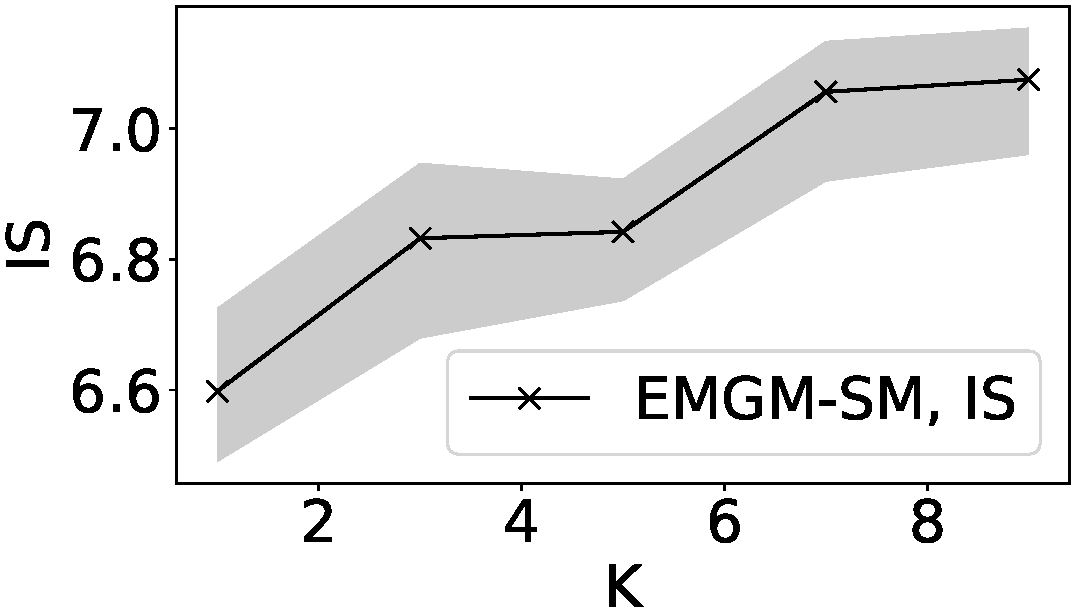
\includegraphics[width=1\linewidth]{images/mnist/scores/EMGM-NM/EMGM-NM-IS-K.pdf}
% %     \caption{IS score}
%     %     \label{fig-nm-isk}
%   \end{subfigure}
%   \vspace{-2pt}
%   \begin{subfigure}{.24\textwidth}
%     \centering
%     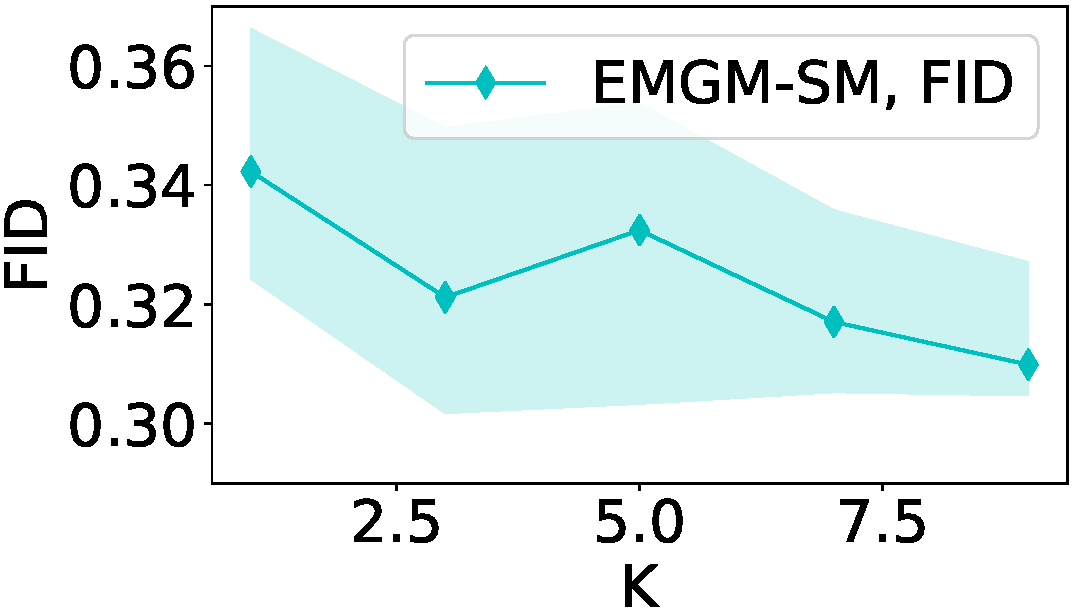
\includegraphics[width=1\linewidth]{images/mnist/scores/EMGM-NM/EMGM-NM-FID-K.pdf}
%     %     \caption{FID score}
%     %     \label{fig-nm-fidk}
%   \end{subfigure}
%   \centering
%   \begin{subfigure}{.24\textwidth}
%     \centering
%     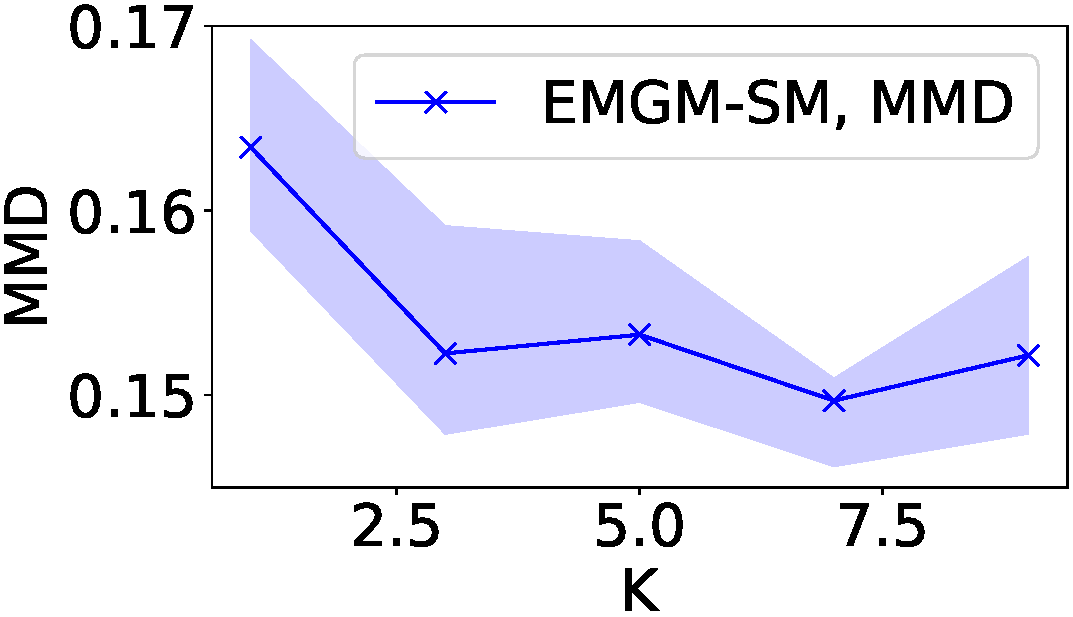
\includegraphics[width=1\linewidth]{images/mnist/scores/EMGM-NM/EMGM-NM-MMD-K.pdf}
%     %     \caption{MMD score}
%     %     \label{fig-nm-mmdk}
%   \end{subfigure}
%   \centering
%   \begin{subfigure}{0.24\textwidth}
%     \centering
%     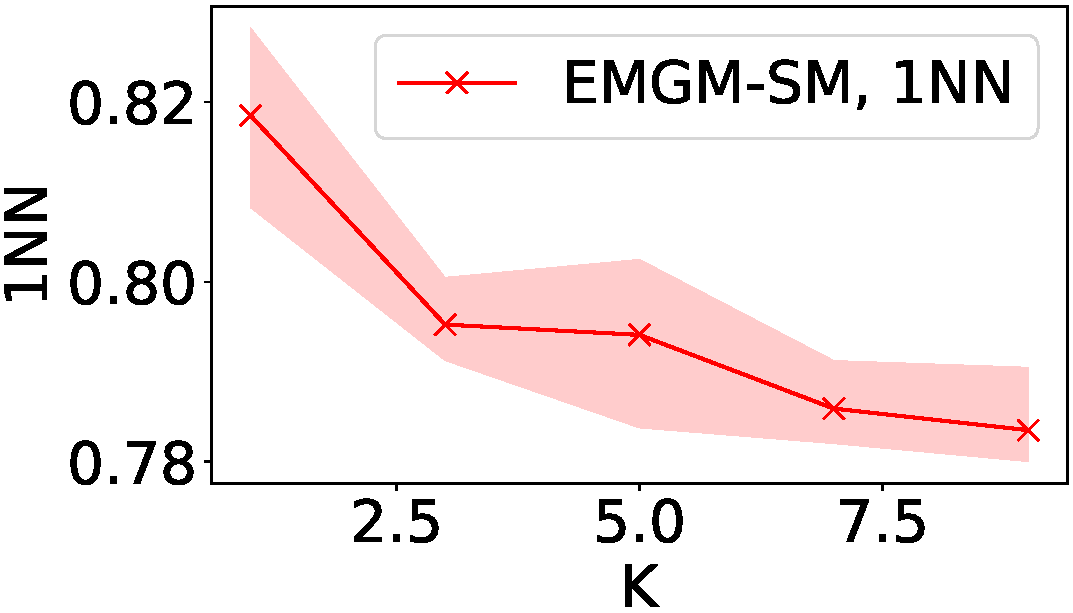
\includegraphics[width=1\linewidth]{images/mnist/scores/EMGM-NM/EMGM-NM-1NN-K.pdf}
%     %     \caption{1NN score}
%     %     \label{fig-nm-1nnk}
%   \end{subfigure}
%   \centering
%   \begin{subfigure}{.24\textwidth}
%     \centering
%     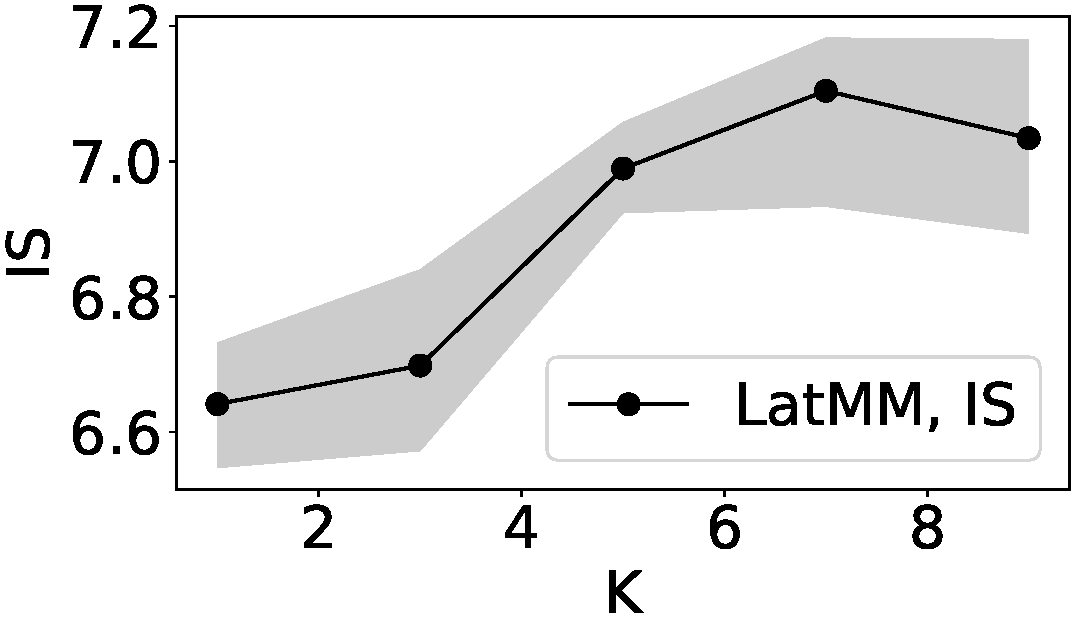
\includegraphics[width=1\linewidth]{images/mnist/scores/EMGM-SM/EMGM-SM-IS-K.pdf}
%     %     \caption{IS score}
%     %     \label{fig-sm-is}
%   \end{subfigure}
%   \centering
%   \begin{subfigure}{.24\textwidth}
%     \centering
%     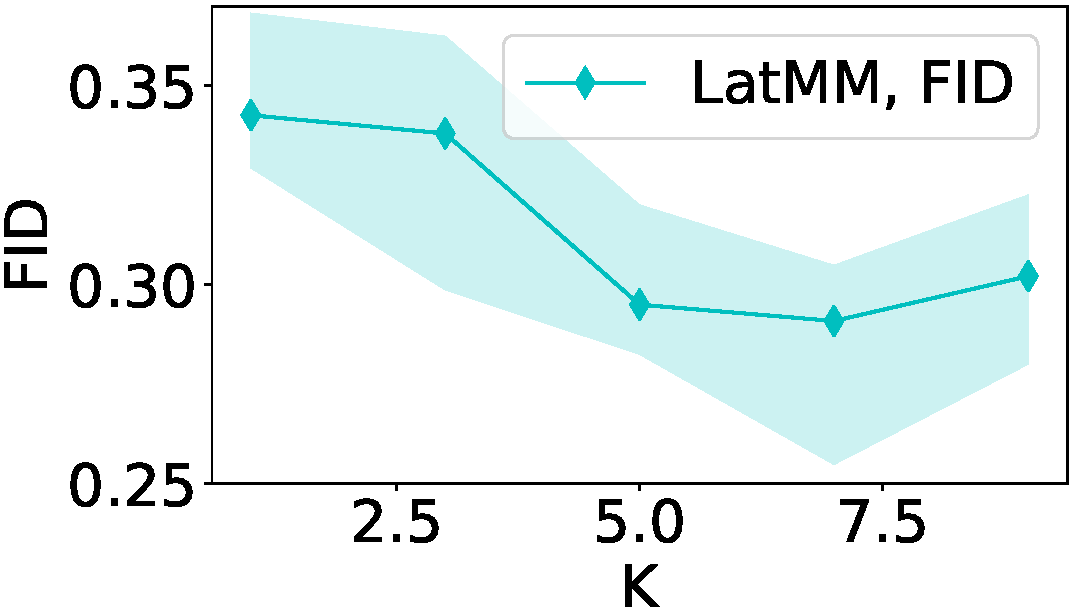
\includegraphics[width=1\linewidth]{images/mnist/scores/EMGM-SM/EMGM-SM-FID-K.pdf}
%     %     \caption{FID score}
%     %     \label{fig-sm-fid}
%   \end{subfigure}
%   \centering
%   \begin{subfigure}{.24\textwidth}
%     \centering
%     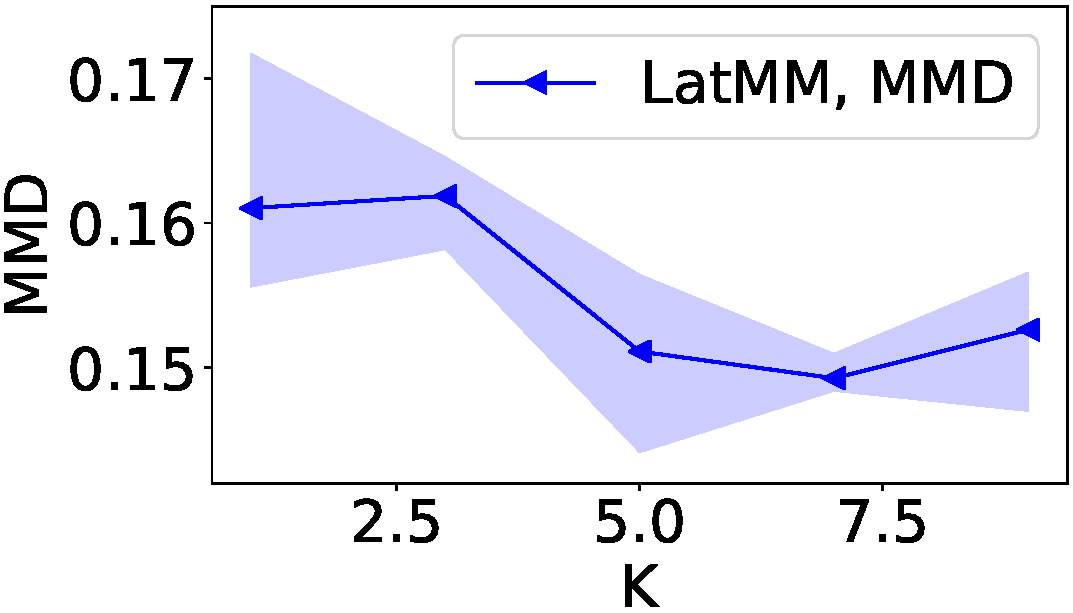
\includegraphics[width=1\linewidth]{images/mnist/scores/EMGM-SM/EMGM-SM-MMD-K.pdf}
%     %     \caption{MMD score}
%     %     \label{fig-sm-mmd}
%   \end{subfigure}
%   \begin{subfigure}{0.24\textwidth}
%     \centering
%     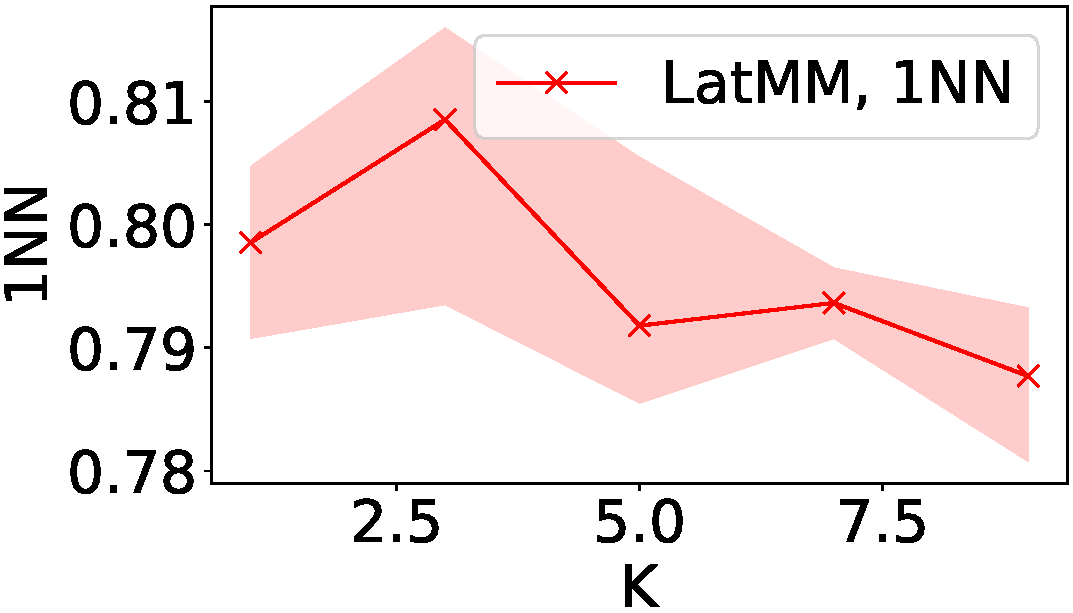
\includegraphics[width=1.\linewidth]{images/mnist/scores/EMGM-SM/EMGM-SM-1NN-K.pdf}
%     %     \caption{1NN score}
%     %     \label{fig-sm-1nn}
%   \end{subfigure}
%   \caption{IS, FID, MMD and 1NN scores of GenMM and LatMM. Evaluated
%   on $2000$ samples ($1000$ samples generated by GenMM or LatMM for
%   corresponding $K$, $1000$ samples from MNIST). $5$ experiments are
%   carried out for each assessed score at each setting of $K$. Curve
%   with marker stands for mean score and shaded area stands for the range of corresponding score. \textcolor{green}{This experiments is rechecked. Reproduced results are similar to what is shown here. (Latent standard Gaussian use standard deviation std =0.8) }}
%   \vspace{10pt}
% \end{figure*}

% \begin{figure*}[!ht]
%   \captionsetup[subfigure]{justification=centering}
%   \centering
%   \begin{subfigure}{.24\textwidth}
%     \centering
%     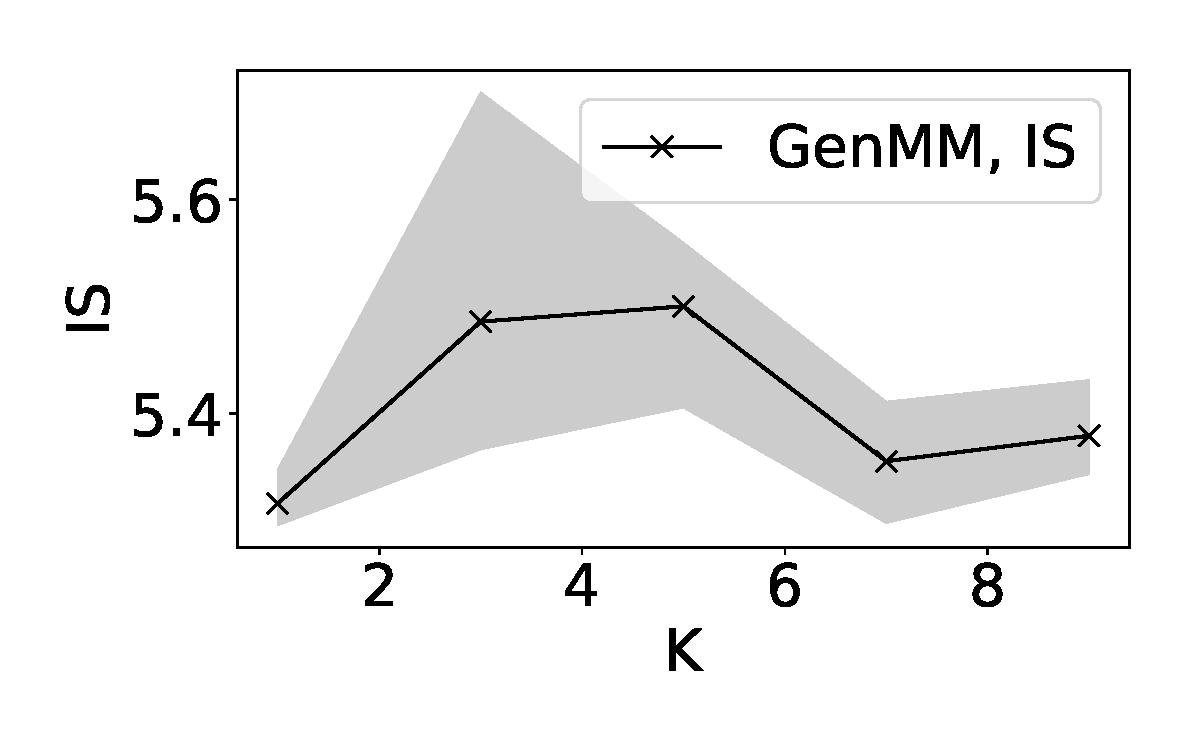
\includegraphics[width=1\linewidth]{images/fashion-mnist/scores/EMGM-NM/EMGM-NM-IS-K.pdf}
% %     \caption{IS score}
%     %     \label{fig-nm-isk}
%   \end{subfigure}
%   \vspace{-2pt}
%   \begin{subfigure}{.24\textwidth}
%     \centering
%     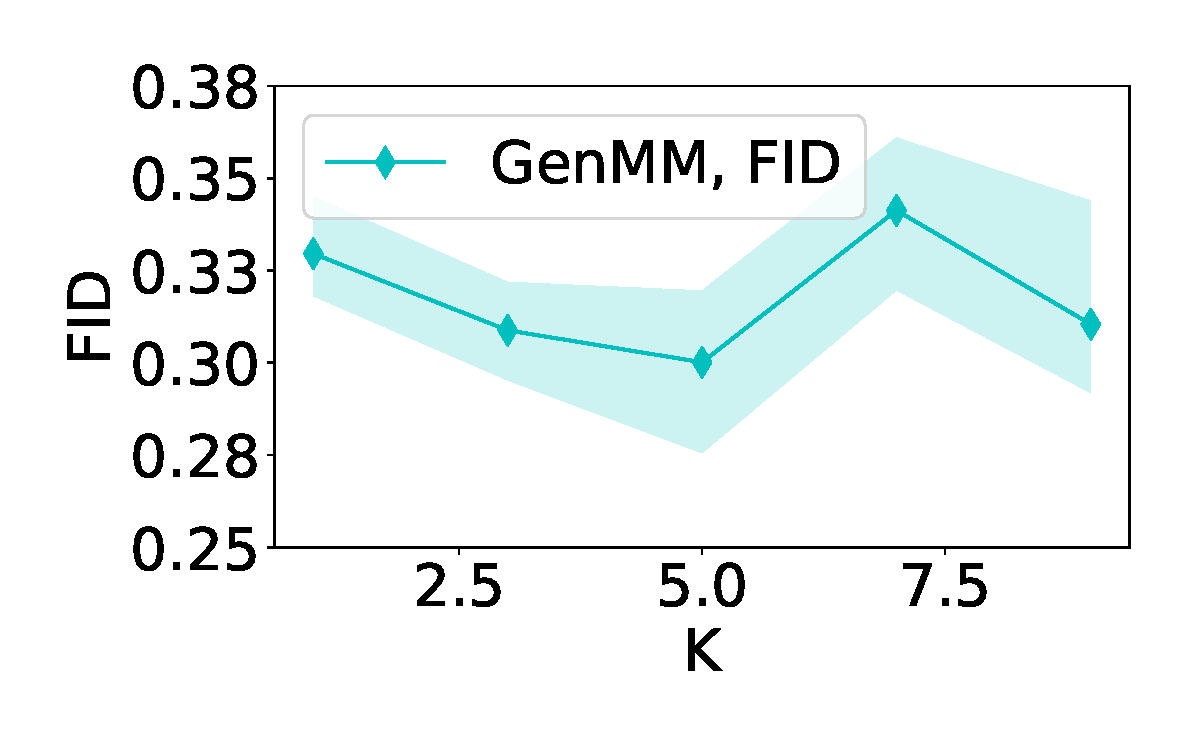
\includegraphics[width=1\linewidth]{images/fashion-mnist/scores/EMGM-NM/EMGM-NM-FID-K.pdf}
%     %     \caption{FID score}
%     %     \label{fig-nm-fidk}
%   \end{subfigure}
%   \centering
%   \begin{subfigure}{.24\textwidth}
%     \centering
%     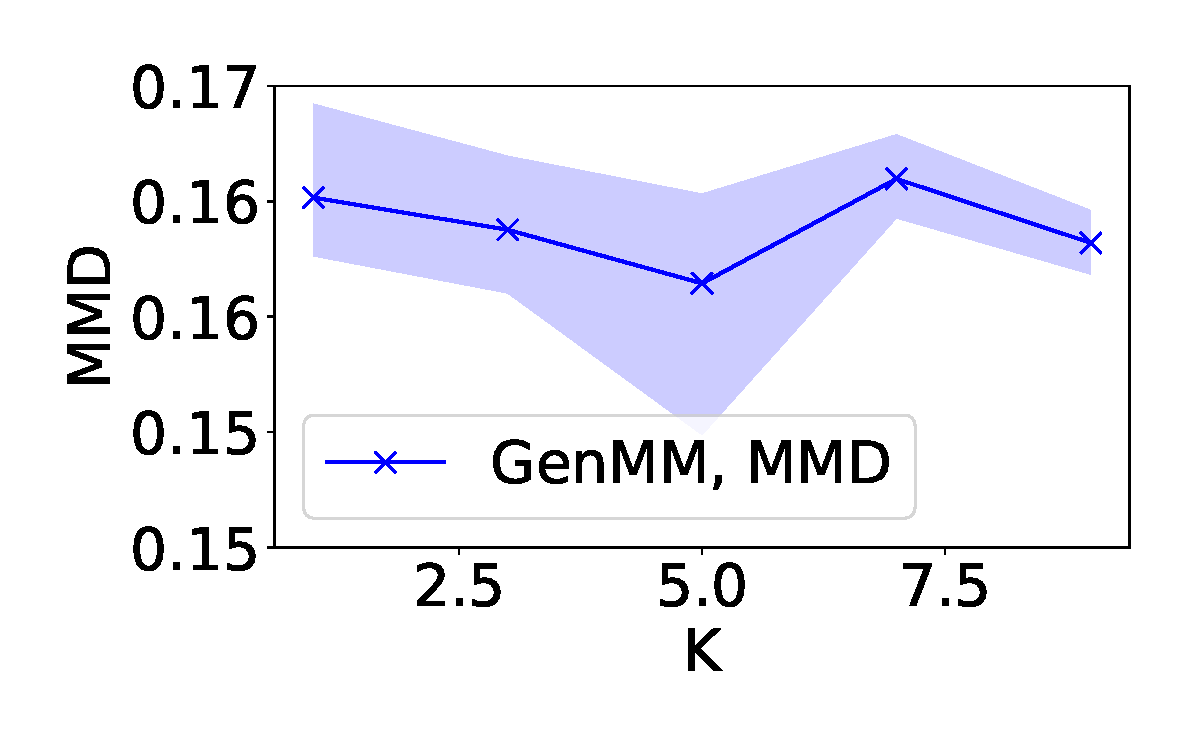
\includegraphics[width=1\linewidth]{images/fashion-mnist/scores/EMGM-NM/EMGM-NM-MMD-K.pdf}
%     %     \caption{MMD score}
%     %     \label{fig-nm-mmdk}
%   \end{subfigure}
%   \centering
%   \begin{subfigure}{0.24\textwidth}
%     \centering
%     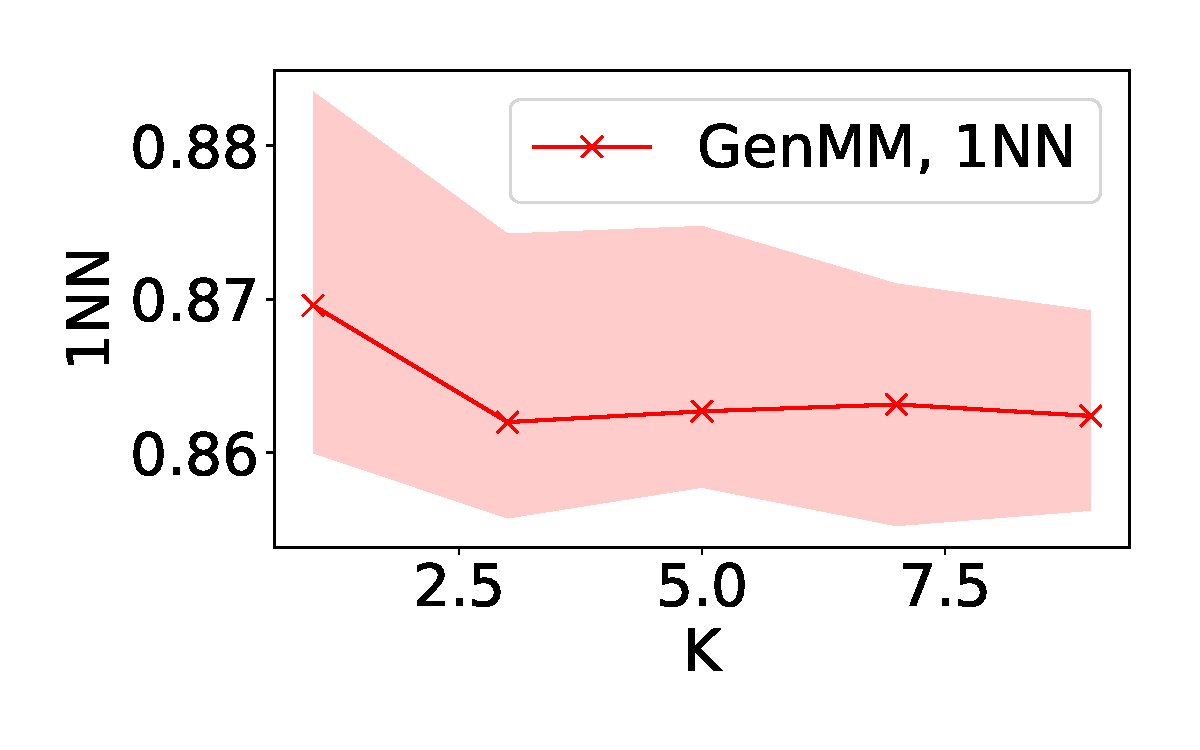
\includegraphics[width=1\linewidth]{images/fashion-mnist/scores/EMGM-NM/EMGM-NM-1NN-K.pdf}
%     %     \caption{1NN score}
%     %     \label{fig-nm-1nnk}
%   \end{subfigure}
%   \centering
%   \begin{subfigure}{.24\textwidth}
%     \centering
%     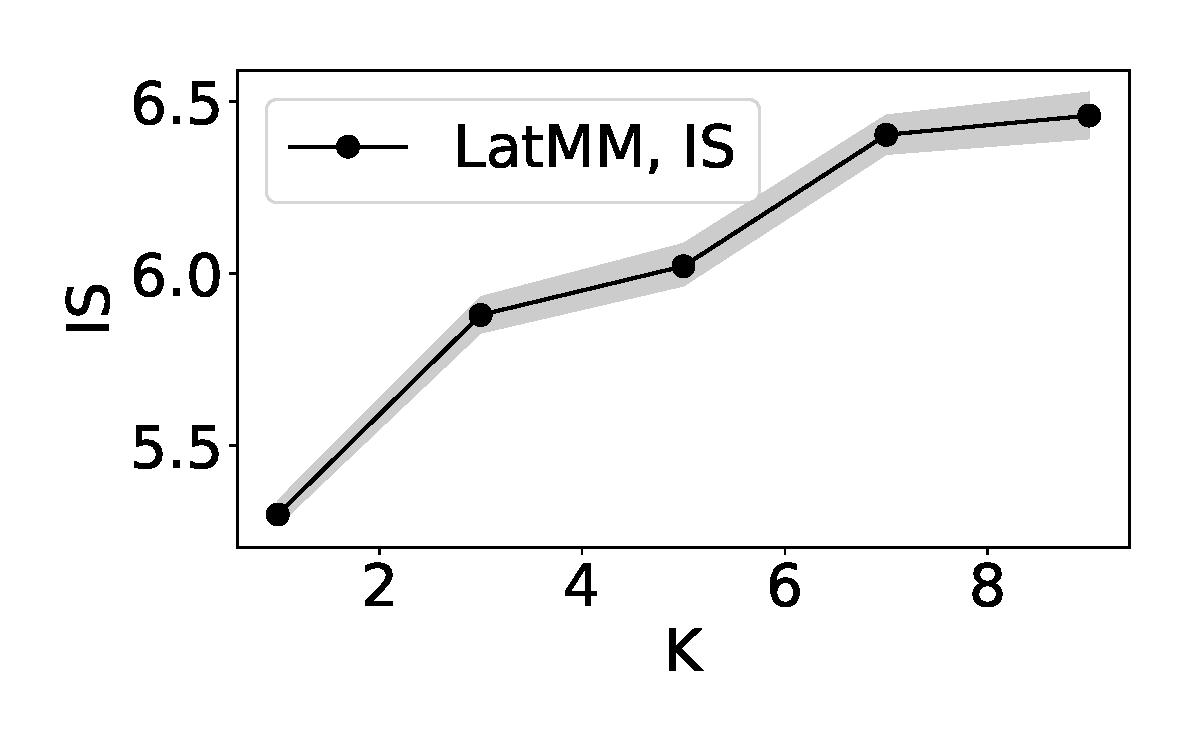
\includegraphics[width=1\linewidth]{images/fashion-mnist/scores/EMGM-SM/EMGM-SM-IS-K.pdf}
%     %     \caption{IS score}
%     %     \label{fig-sm-is}
%   \end{subfigure}
%   \centering
%   \begin{subfigure}{.24\textwidth}
%     \centering
%     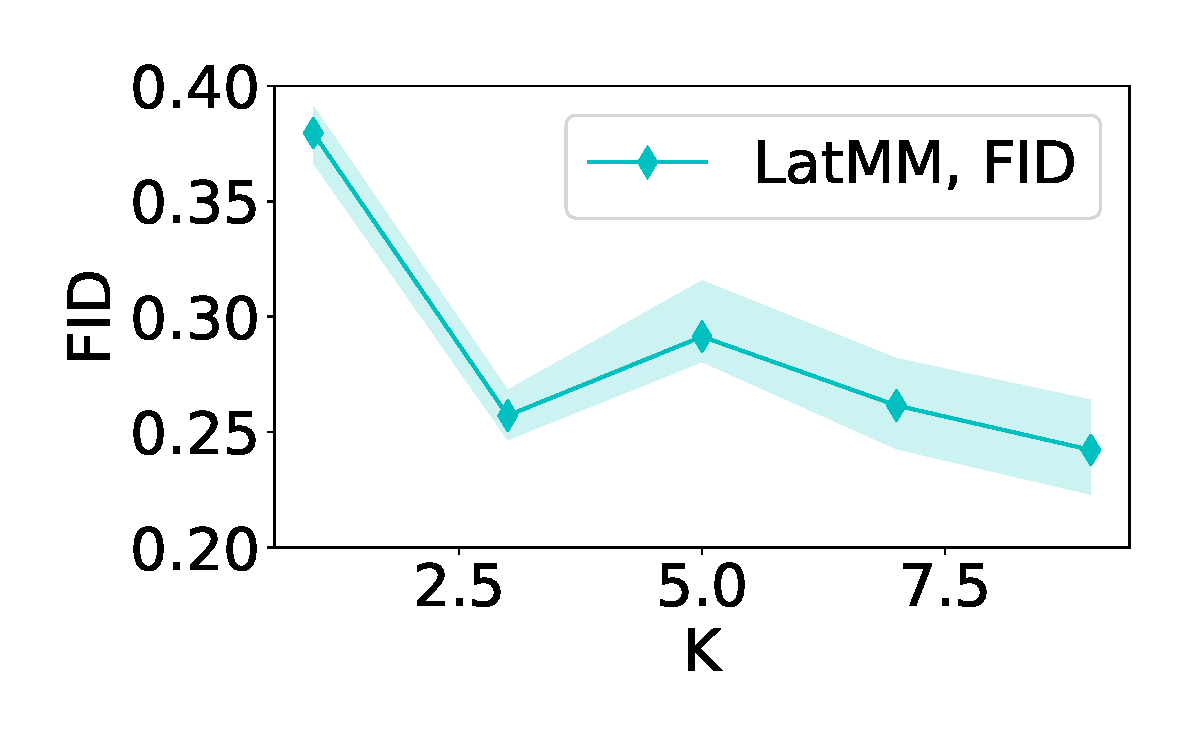
\includegraphics[width=1\linewidth]{images/fashion-mnist/scores/EMGM-SM/EMGM-SM-FID-K.pdf}
%     %     \caption{FID score}
%     %     \label{fig-sm-fid}
%   \end{subfigure}
%   \centering
%   \begin{subfigure}{.24\textwidth}
%     \centering
%     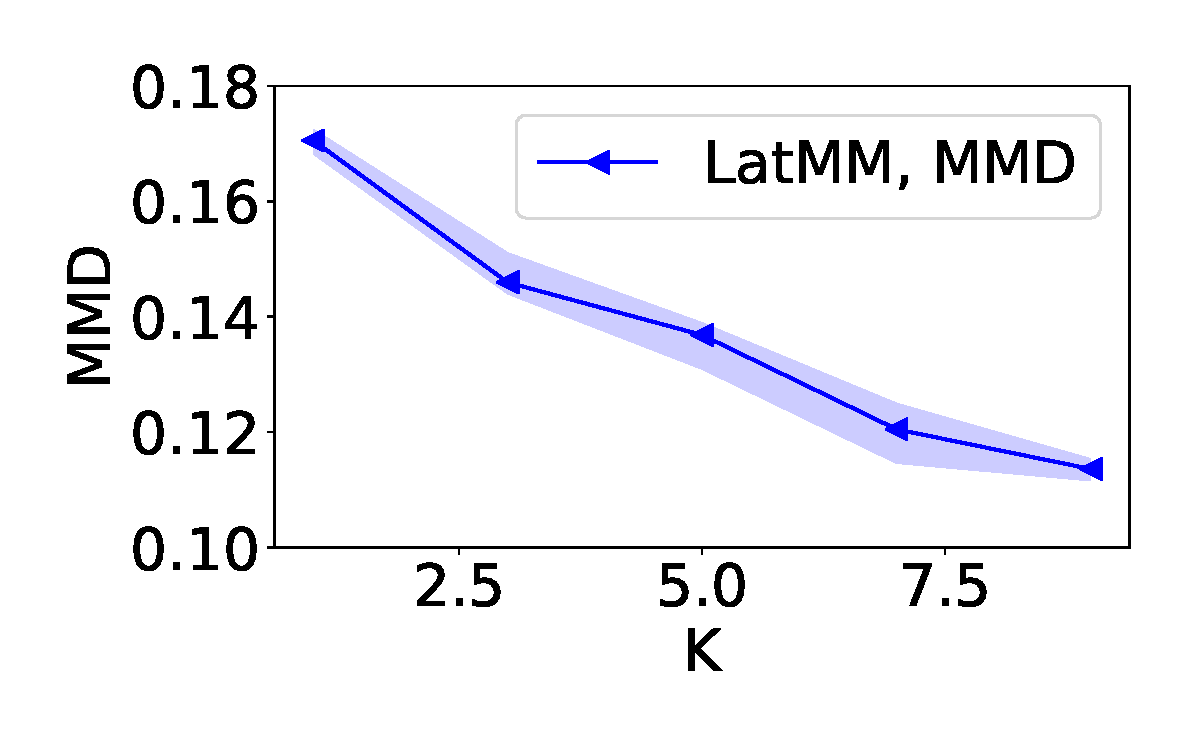
\includegraphics[width=1\linewidth]{images/fashion-mnist/scores/EMGM-SM/EMGM-SM-MMD-K.pdf}
%     %     \caption{MMD score}
%     %     \label{fig-sm-mmd}
%   \end{subfigure}
%   \begin{subfigure}{0.24\textwidth}
%     \centering
%     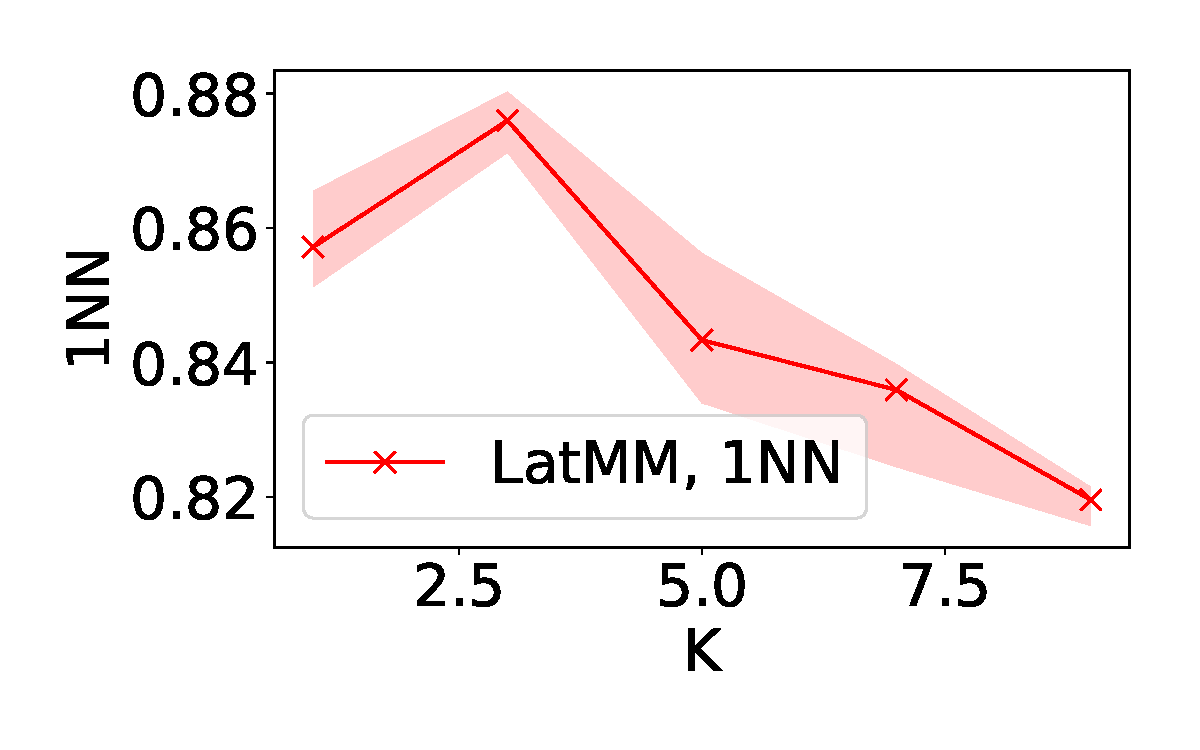
\includegraphics[width=1.\linewidth]{images/fashion-mnist/scores/EMGM-SM/EMGM-SM-1NN-K.pdf}
%     %     \caption{1NN score}
%     %     \label{fig-sm-1nn}
%   \end{subfigure}
%   \caption{ GenMM and LatMM evaluated on Fashion-MNIST (std =0.8) }
%   \vspace{10pt}
% \end{figure*}



In this section, we evaluate our proposed mixture models for generating samples and maximum likelihood classification. We will show encouraging results.

% under different metrics firstly. Then demos of sample generating and interpolation are shown. Lastly, we apply our model to classification tasks based on maximum likelihood criterion.

\begin{figure*}[!t]
  \captionsetup[subfigure]{justification=centering}
  \centering
  \begin{subfigure}{.4\textwidth}
    \centering
    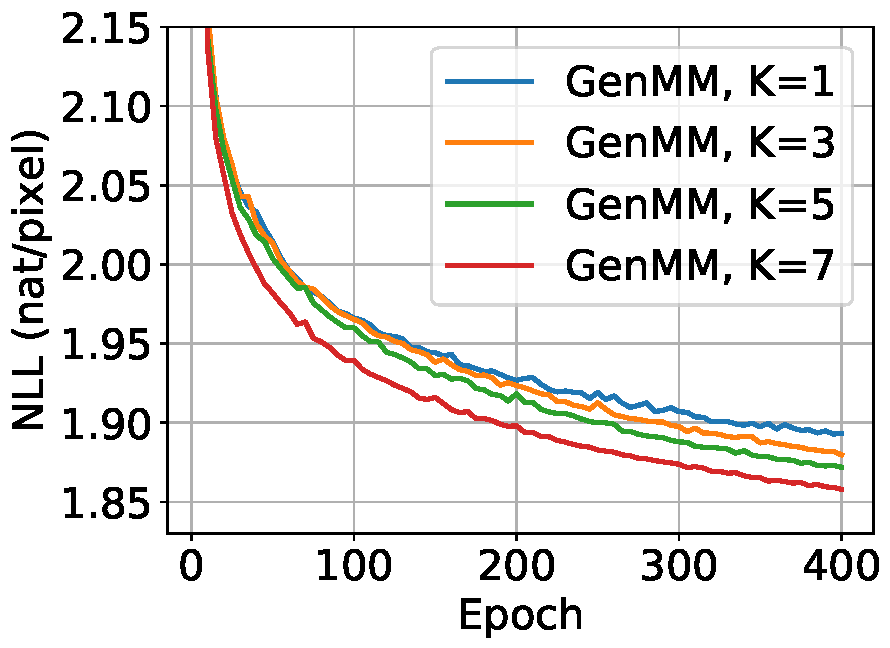
\includegraphics[width=1\linewidth]{images/supply/mnist_GenMM_nll_curves-crop.pdf}
    
    \caption{Dataset MNIST}
    \label{fig-genmm-mnist-nll-curve}
  \end{subfigure}\hspace{1cm}
  \begin{subfigure}{.4\textwidth}
    \centering
    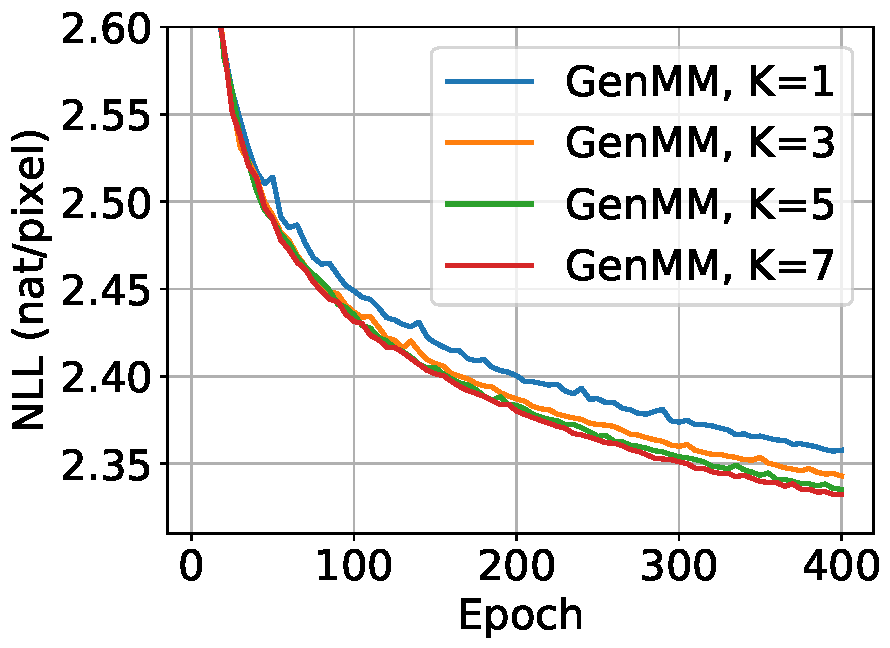
\includegraphics[width=1\linewidth]{images/supply/fashion_GenMM_nll_curves-crop.pdf}
    
    \caption{Dataset Fashion-MNIST}
    \label{fig-genmm-fsh-nll-curve}
  \end{subfigure}
  \caption{NLL (Unit: nat/pixel) of GenMM versus training epochs with different number of mixture component $k$. (a) $10000$ images from MNIST is used for training, (b) $10000$ images from Fashion-MNIST is used for training.}
  \label{fig:genmm-nll}
\end{figure*}

\begin{figure*}[!tp]
  \captionsetup[subfigure]{justification=centering}
  \centering
  \begin{subfigure}{.4\textwidth}
    \centering
    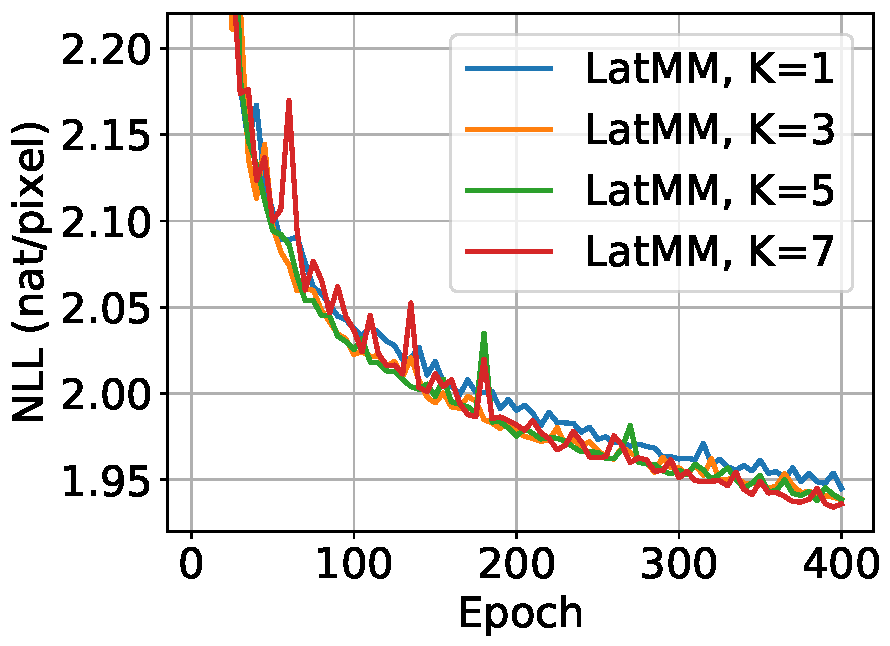
\includegraphics[width=1\linewidth]{images/supply/mnist_LatMM_nll_curves-crop.pdf}
    
    \caption{Dataset of MNIST}
    \label{fig-latmm-mnist-nll-curve}
  \end{subfigure}\hspace{1cm}
  \begin{subfigure}{.4\textwidth}
    \centering
    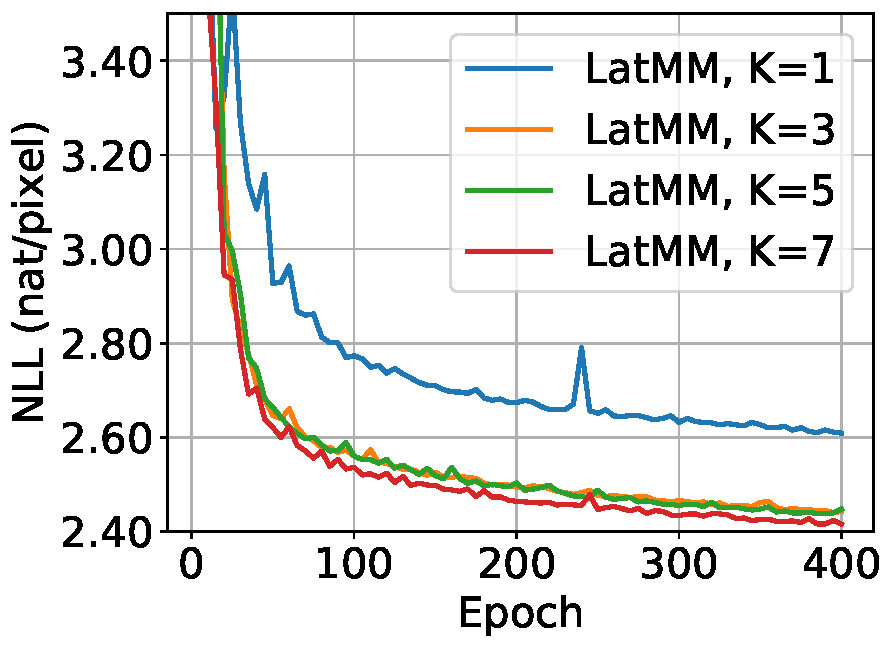
\includegraphics[width=1\linewidth]{images/supply/fashion_LatMM_nll_curves-crop.pdf}
    
    \caption{Dataset Fashion-MNIST}
    \label{fig-latmm-fsh-nll-curve}
  \end{subfigure}
  
  \caption{NLL (Unit: nat/pixel) of LatMM versus training epochs with different number of mixture component $k$. (a) $10000$ images from MNIST is used for training, (b) $10000$ images from Fashion-MNIST is used for training.}
  \label{fig:latmm-nll}
\end{figure*}


\subsection{Experimental setup}\label{sub:exp-setup}

We use the flow-based neural network for implementing generators $\{\bm{g}_k\}_{k=1}^{K}$ in GenMM and $\bm{g}$ in LatMM. Specifically, we use the Glow structure \cite{2018arXiv180703039K} that is developed based on RealNVP \cite{2016arXiv160508803D} and NICE \cite{DBLP:journals/corr/DinhKB14}. As introduced in section~\ref{chpt6:sec:flow}, the operation in \eqref{eq-gl} is a coupling
layer. Since only a part of the input is mapped non-linearly after a coupling
layer and the rest part remains the same, permutation \cite{2016arXiv160508803D} or $1\times 1$ convolution operation \cite{2018arXiv180703039K} is used to alternate the part of signal that goes through identity mapping. In Glow structure, a basic \textit{flow step} is the concatenation of three layers: Actnorm (element-wise affine mapping)
$\rightarrow$ $1\times 1$ Convolution (for permutation purpose)
$\rightarrow$ Coupling layer. A \textit{flow block} consists of: a squeeze layer,
several flow steps, a split layer. A squeeze layer reshapes
signal. A split layer allows
flow model to split some elements of hidden layers out and model them
directly as standard Gaussian, which relieves computation burden. In our experiments, there are also split layers that make dimension of $\bm{z}$ one fourth of dimension $\bm{x}$, and split signal in hidden layers are modeled as standard Gaussian. 

% In all of our experiments, the generators $\bm{g}_k, \forall k$, in
% GenMM and $\bm{g}$ of LatMM use the same structure: \textit{three} flow blocks with
% each flow block consisting of \textit{four} coupling layers.  
All generators used in our experiments are randomly initialized before training. 
% In order to make comparison fair, our models with different configuration of $K$ are all trained for $30$ epochs on both datasets. Comparison are made with the trained models.  
In addition, the prior distribution $\bm{\pi}$ update in both GenMM and LatMM is every $5$ epochs, {i.e.},  $t_{\pi} = 5$. For the training of LatMM, we adopt the Gamma distribution $\Gamma(\bm{\sigma}_k^{-1}; a, b)$ as the parameter prior for $\bm{\sigma}_k^{-1}, \forall k$, with shape parameter $a=2$ and rate parameter $b = 1$.

\begin{figure*}[!tp]
  \captionsetup[subfigure]{justification=centering}
  \centering
  \begin{subfigure}{.24\textwidth}
    \centering
    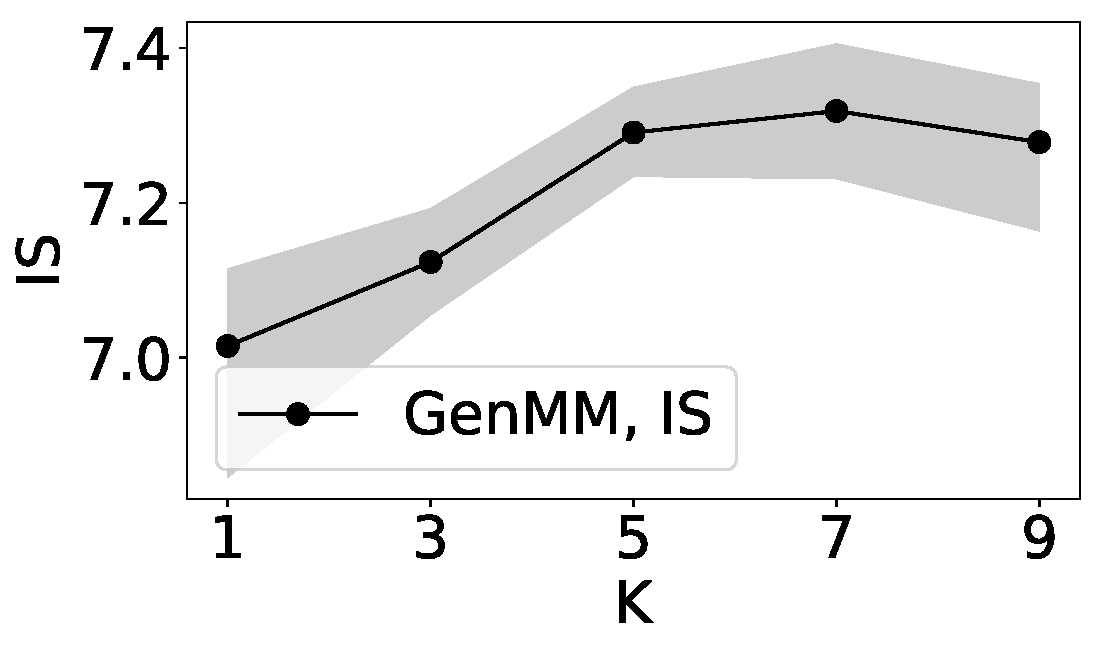
\includegraphics[width=1\linewidth]{images/mnist/scores/std1EMGM-NM/EMGM-NM-IS-K.pdf}
    % \caption{IS score}
    % \label{fig-nm-isk}
  \end{subfigure}
  \vspace{-2pt}
  \begin{subfigure}{.24\textwidth}
    \centering
    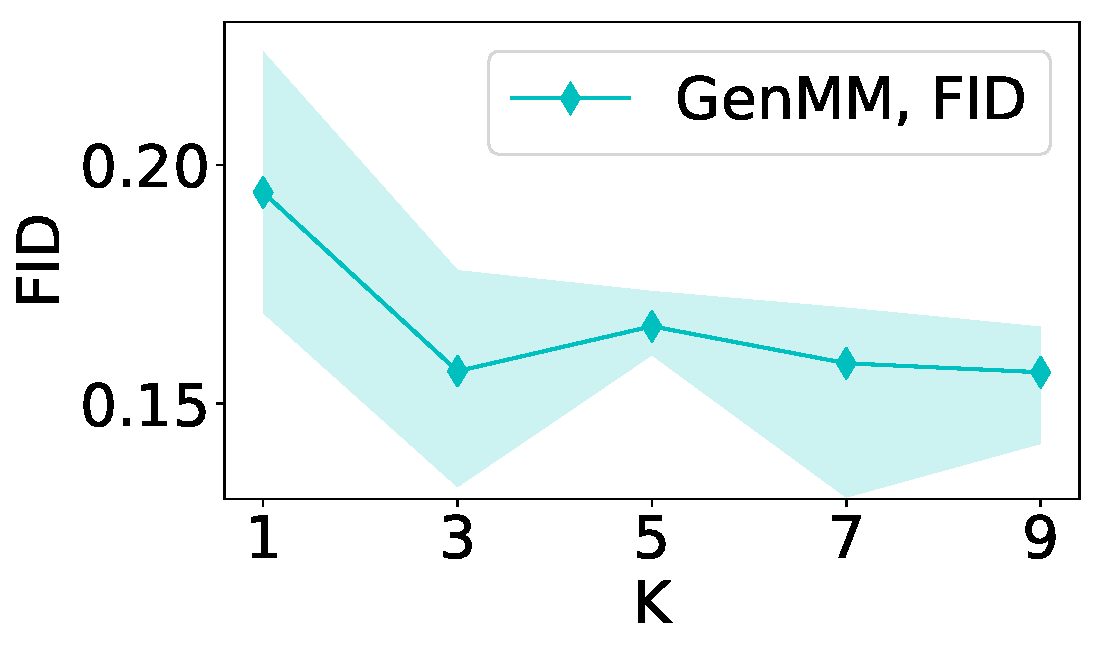
\includegraphics[width=1\linewidth]{images/mnist/scores/std1EMGM-NM/EMGM-NM-FID-K.pdf}
    % \caption{FID score}
    % \label{fig-nm-fidk}
  \end{subfigure}
  \centering
  \begin{subfigure}{.24\textwidth}
    \centering
    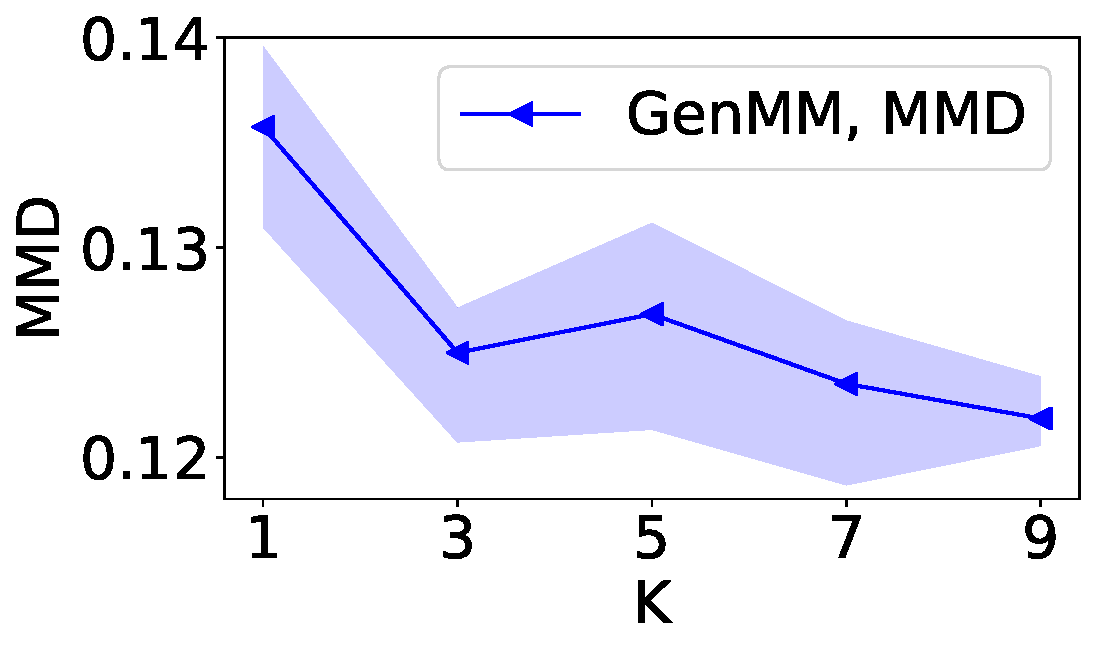
\includegraphics[width=1\linewidth]{images/mnist/scores/std1EMGM-NM/EMGM-NM-MMD-K.pdf}
    % \caption{MMD score}
    % \label{fig-nm-mmdk}
  \end{subfigure}
  \centering
  \begin{subfigure}{0.24\textwidth}
    \centering
    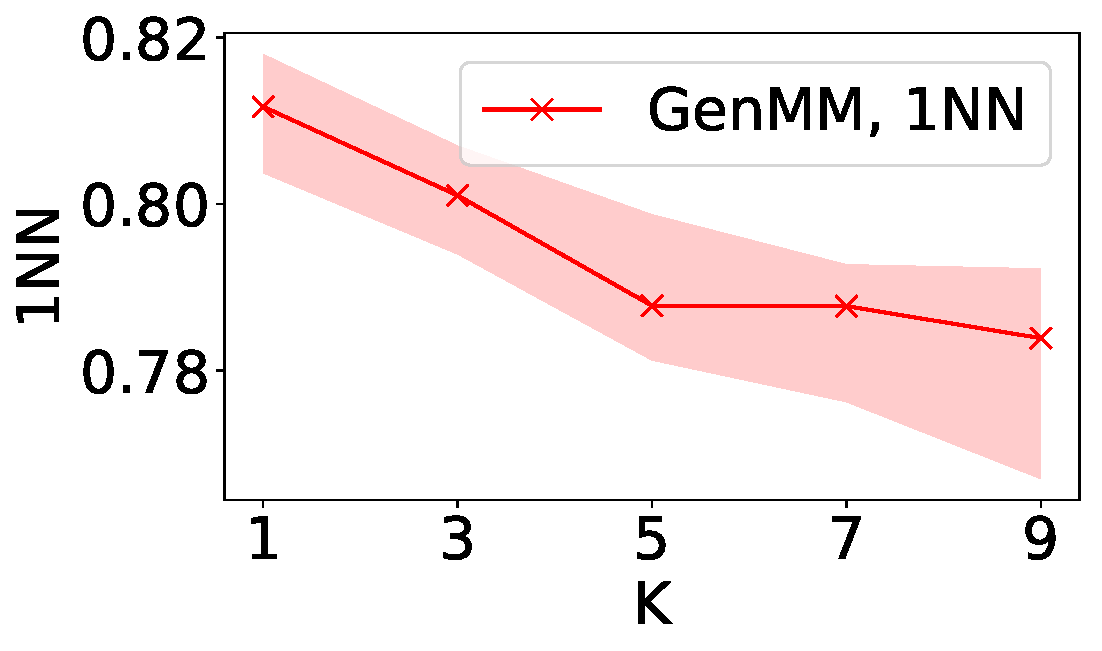
\includegraphics[width=1\linewidth]{images/mnist/scores/std1EMGM-NM/EMGM-NM-1NN-K.pdf}
    % \caption{1NN score}
    % \label{fig-nm-1nnk}
  \end{subfigure}
  \centering
  \begin{subfigure}{.24\textwidth}
    \centering
    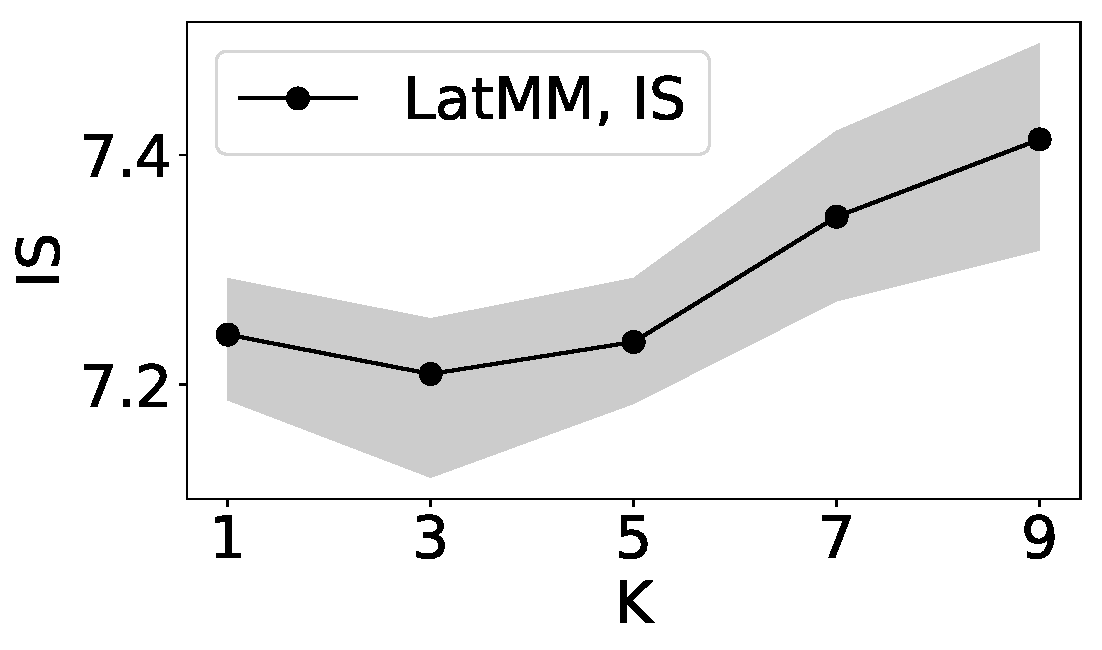
\includegraphics[width=1\linewidth]{images/mnist/scores/std1EMGM-SM/EMGM-SM-IS-K.pdf}
    % \caption{IS score}
    % \label{fig-sm-is}
  \end{subfigure}
  \centering
  \begin{subfigure}{.24\textwidth}
    \centering
    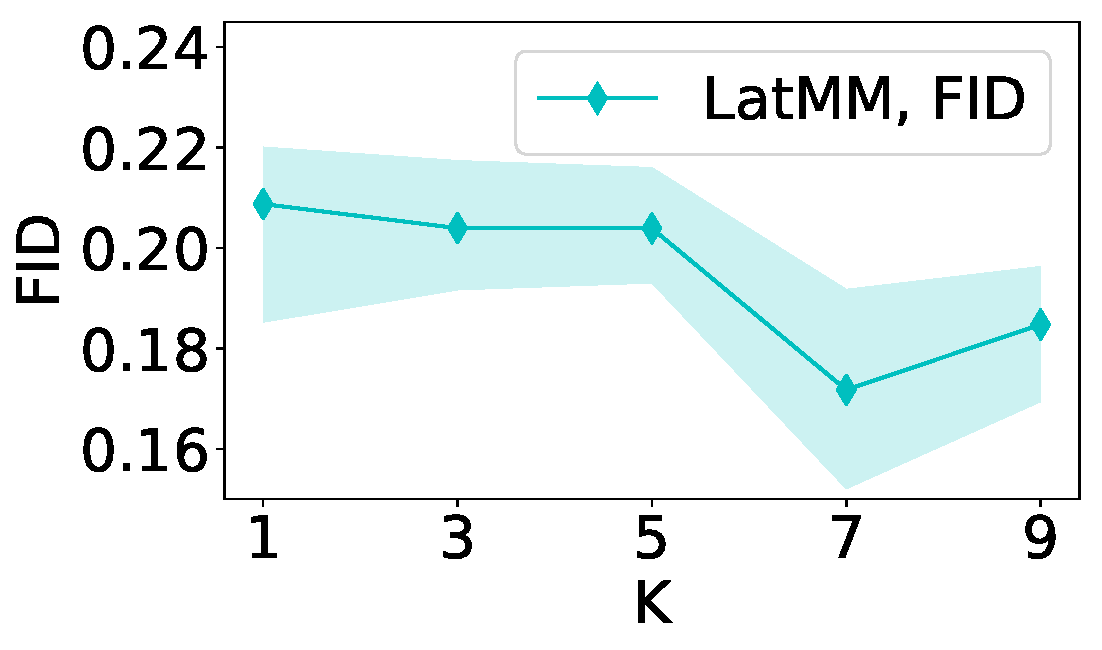
\includegraphics[width=1\linewidth]{images/mnist/scores/std1EMGM-SM/EMGM-SM-FID-K.pdf}
    % \caption{FID score}
    % \label{fig-sm-fid}
  \end{subfigure}
  \centering
  \begin{subfigure}{.24\textwidth}
    \centering
    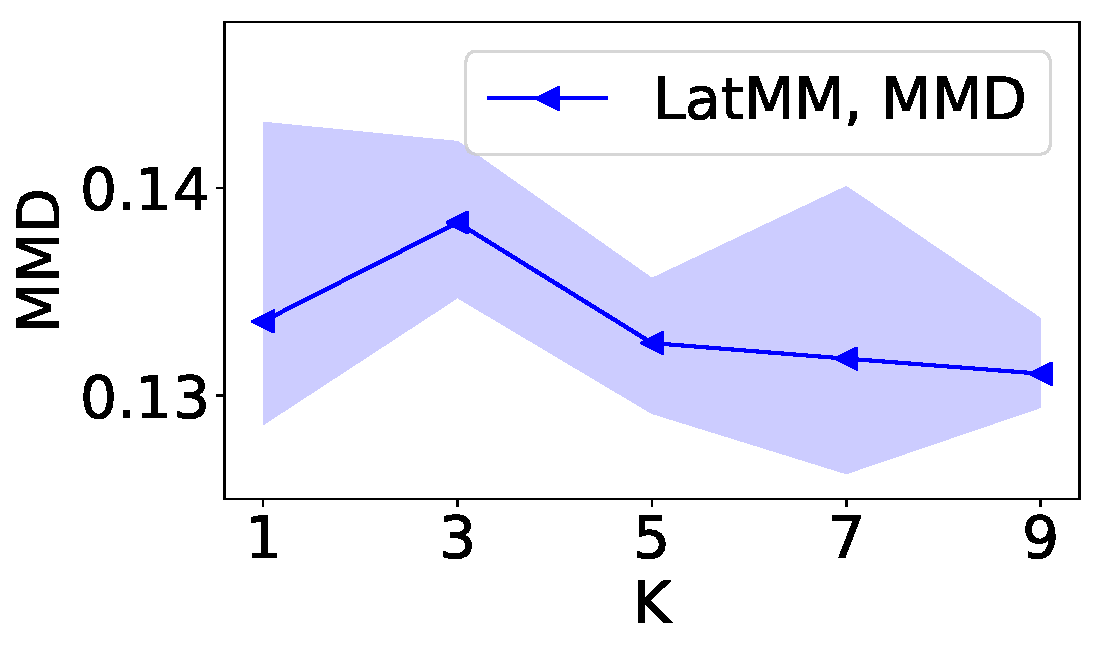
\includegraphics[width=1\linewidth]{images/mnist/scores/std1EMGM-SM/EMGM-SM-MMD-K.pdf}
    % \caption{MMD score}
    % \label{fig-sm-mmd}
  \end{subfigure}
  \begin{subfigure}{0.24\textwidth}
    \centering
    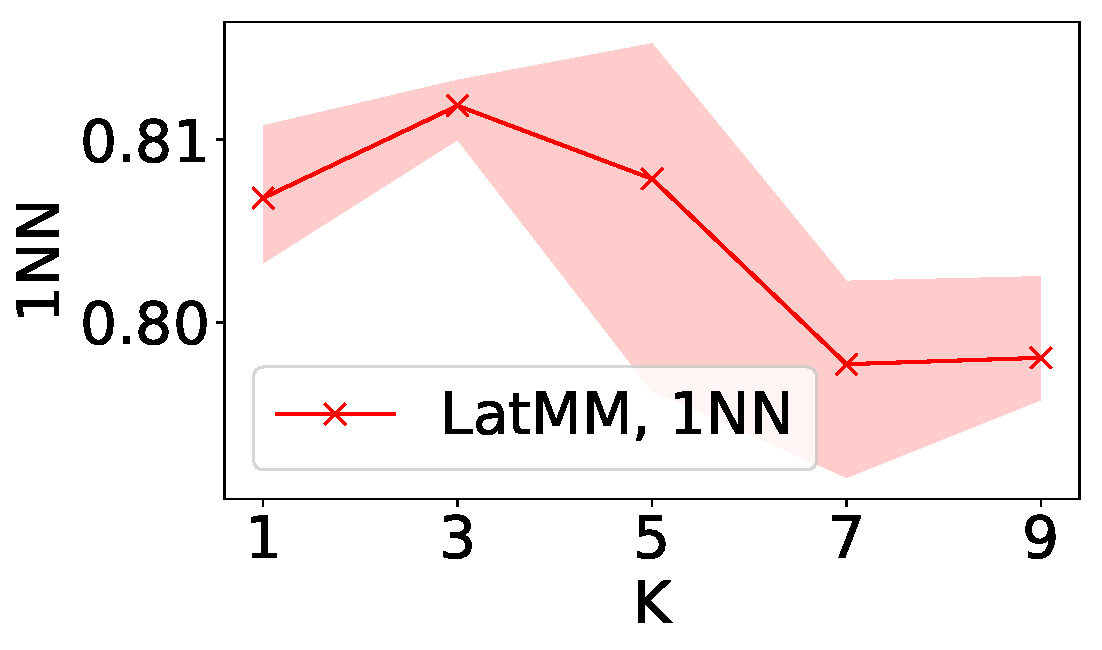
\includegraphics[width=1.\linewidth]{images/mnist/scores/std1EMGM-SM/EMGM-SM-1NN-K.pdf}
    % \caption{1NN score}
    % \label{fig-sm-1nn}
  \end{subfigure}
  \caption{IS, FID, MMD and 1NN of GenMM and LatMM for MNIST dataset. GenMM and LatMM are trained on $60000$ images of MNIST. The results are evaluated on $2000$ samples per simulation point ($1000$ samples generated by GenMM or LatMM for corresponding $K$, $1000$ samples from MNIST). $5$ experiments are carried out for each assessed score at each setting of $K$. Curve with marker denotes mean score and shaded area denotes the range of corresponding score.}\label{fig-scores-k}
\end{figure*}

\begin{figure*}[!ht]
  \captionsetup[subfigure]{justification=centering}
  \centering
  \begin{subfigure}{.24\textwidth}
    \centering
    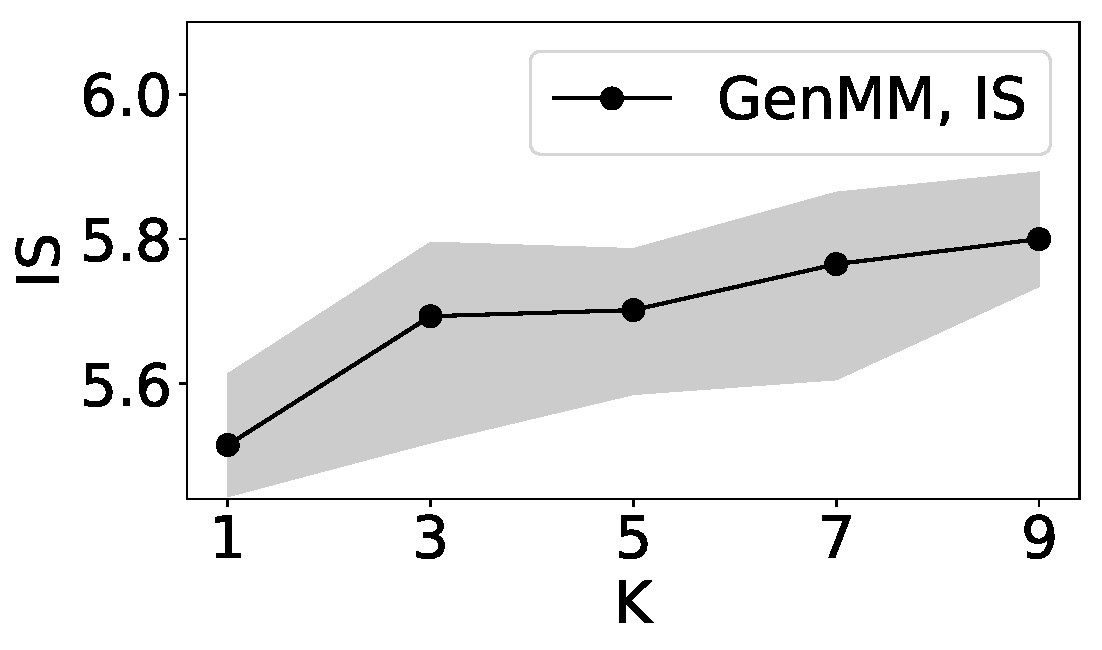
\includegraphics[width=1.0\linewidth]{images/fashion-mnist/scores/std1EMGM-NM/EMGM-NM-IS-K.pdf}
    % \caption{IS score}
    % \label{fig-nm-isk}
  \end{subfigure}
  \vspace{-2pt}
  \begin{subfigure}{.24\textwidth}
    \centering
    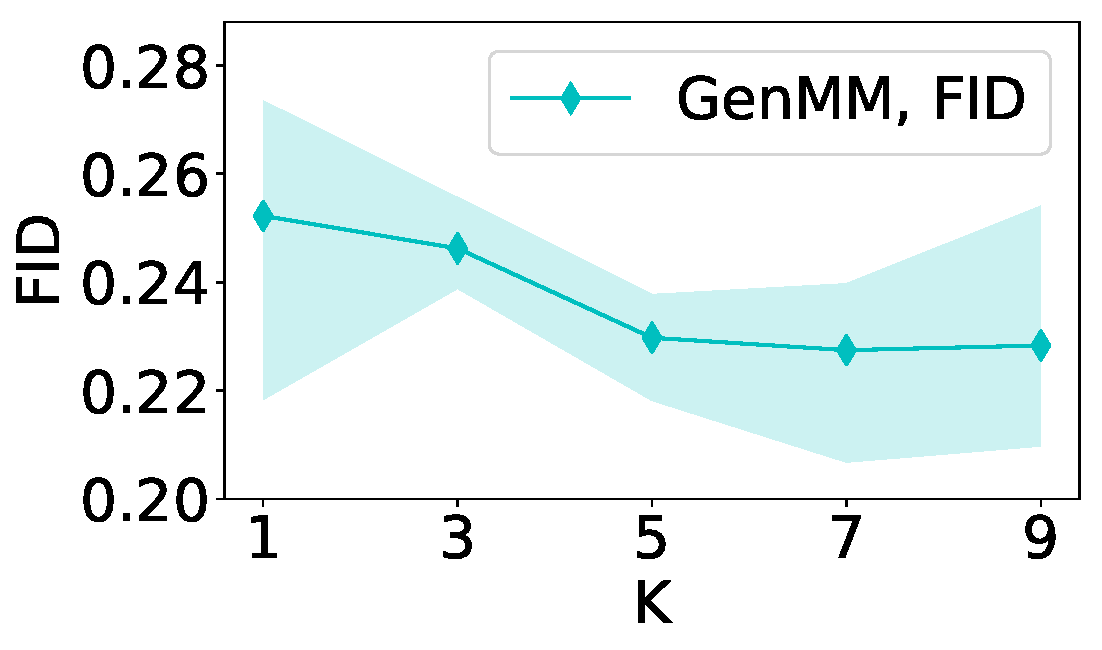
\includegraphics[width=1.0\linewidth]{images/fashion-mnist/scores/std1EMGM-NM/EMGM-NM-FID-K.pdf}
    % \caption{FID score}
    % \label{fig-nm-fidk}
  \end{subfigure}
  \centering
  \begin{subfigure}{.24\textwidth}
    \centering
    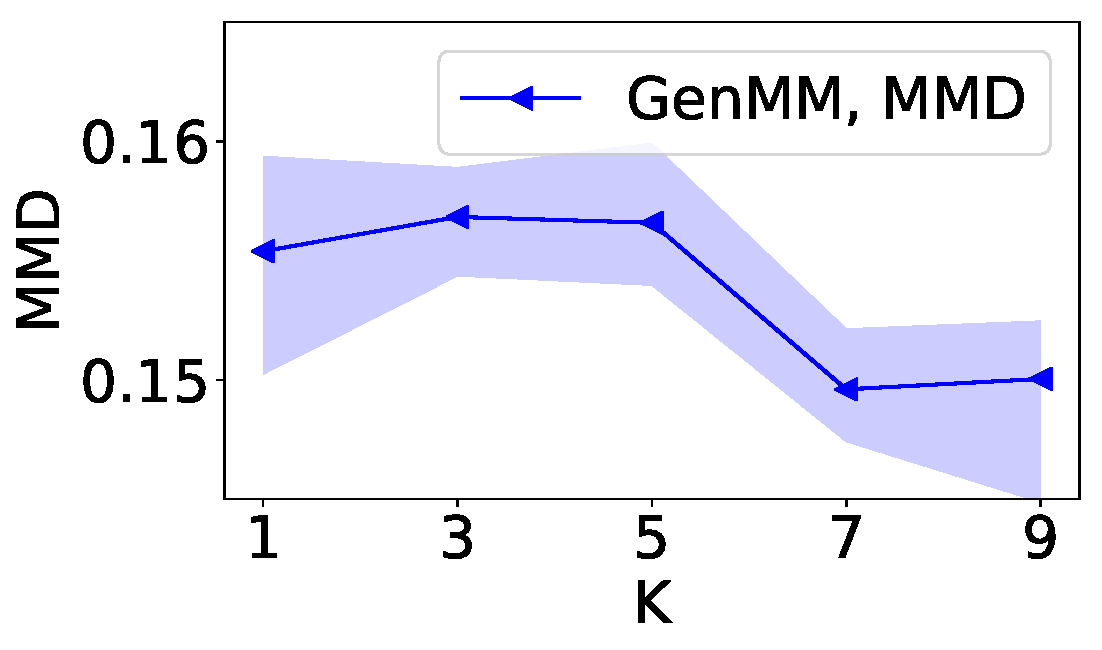
\includegraphics[width=1\linewidth]{images/fashion-mnist/scores/std1EMGM-NM/EMGM-NM-MMD-K.pdf}
    % \caption{MMD score}
    % \label{fig-nm-mmdk}
  \end{subfigure}
  \centering
  \begin{subfigure}{0.24\textwidth}
    \centering
    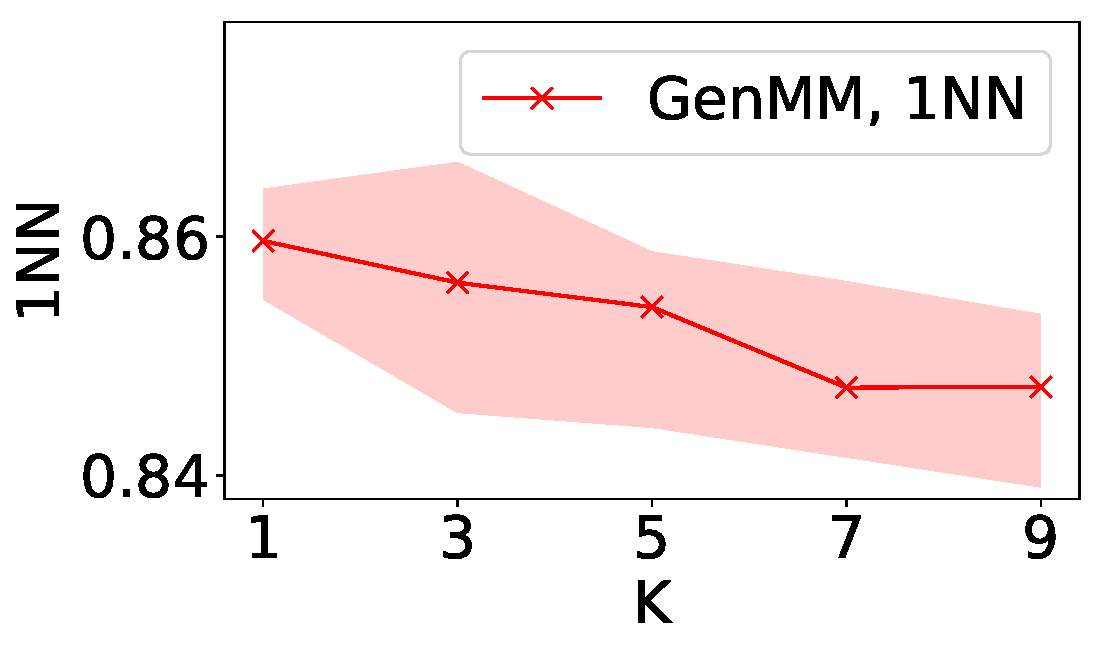
\includegraphics[width=1\linewidth]{images/fashion-mnist/scores/std1EMGM-NM/EMGM-NM-1NN-K.pdf}
    % \caption{1NN score}
    % \label{fig-nm-1nnk}
  \end{subfigure}
  \centering
  \begin{subfigure}{.24\textwidth}
    \centering
    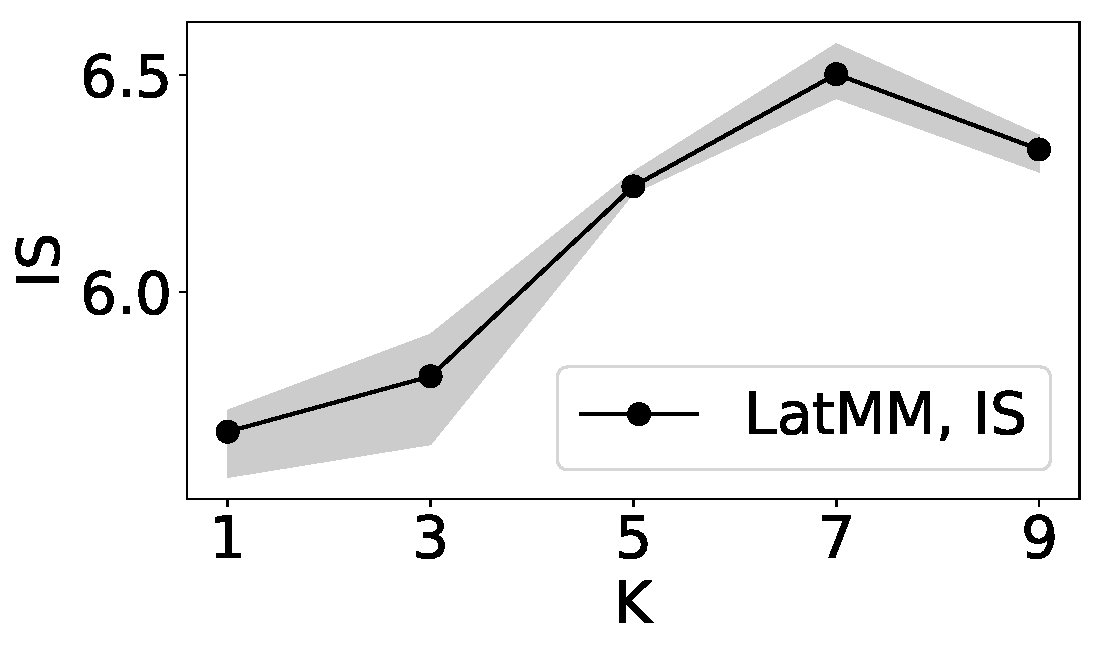
\includegraphics[width=1\linewidth]{images/fashion-mnist/scores/std1EMGM-SM/EMGM-SM-IS-K.pdf}
    % \caption{IS score}
    % \label{fig-sm-is}
  \end{subfigure}
  \centering
  \begin{subfigure}{.24\textwidth}
    \centering
    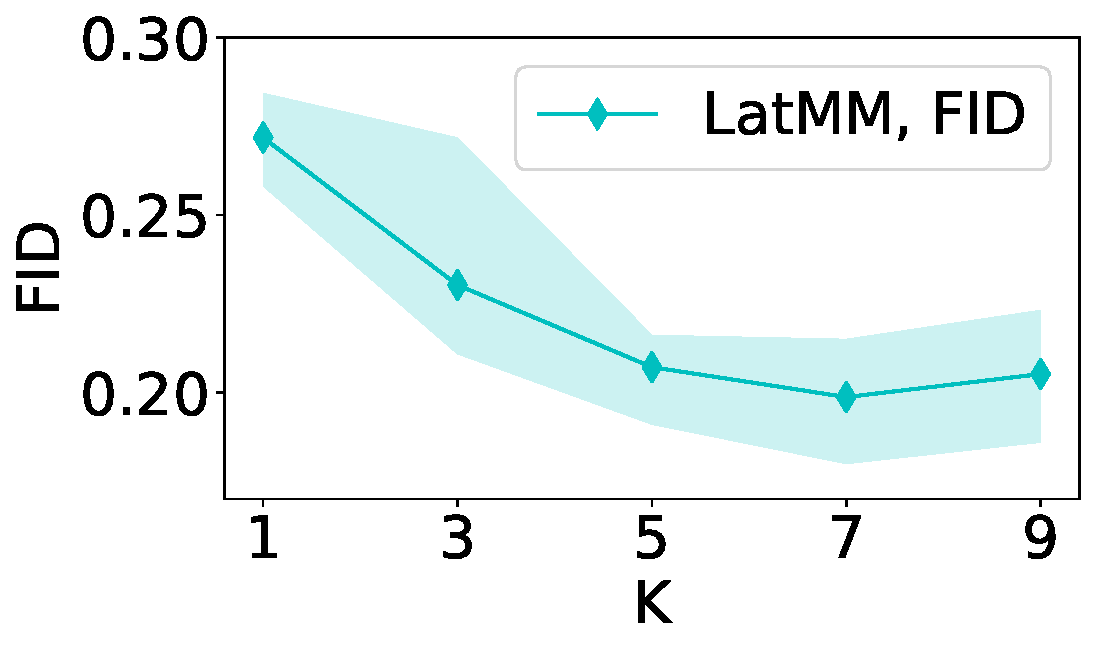
\includegraphics[width=1\linewidth]{images/fashion-mnist/scores/std1EMGM-SM/EMGM-SM-FID-K.pdf}
    % \caption{FID score}
    % \label{fig-sm-fid}
  \end{subfigure}
  \centering
  \begin{subfigure}{.24\textwidth}
    \centering
    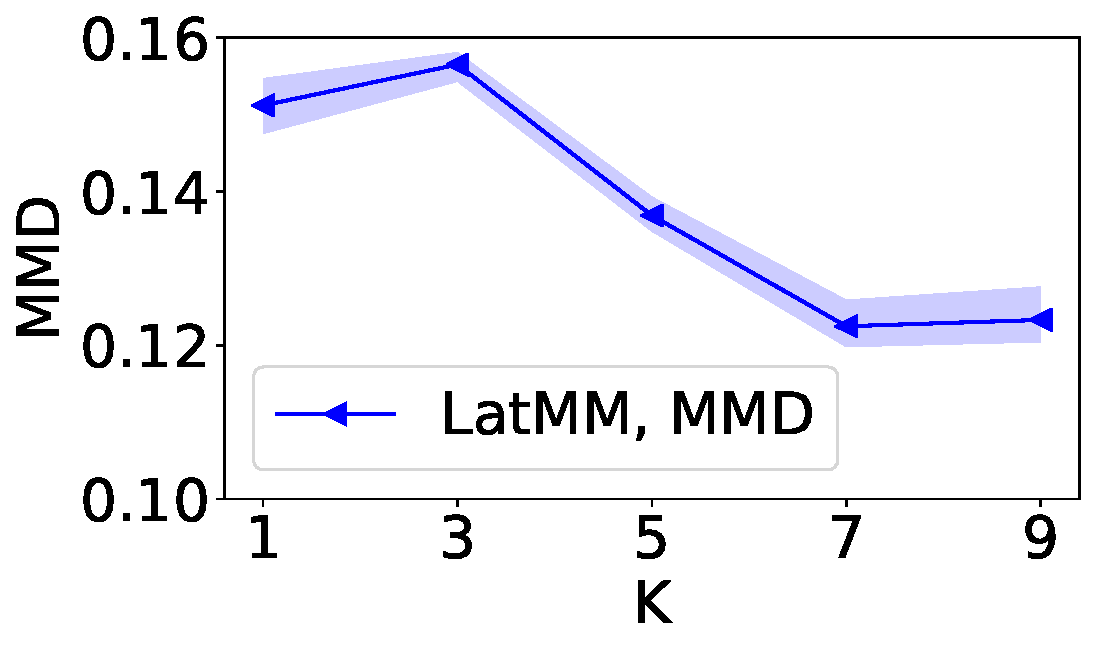
\includegraphics[width=1\linewidth]{images/fashion-mnist/scores/std1EMGM-SM/EMGM-SM-MMD-K.pdf}
    % \caption{MMD score}
    % \label{fig-sm-mmd}
  \end{subfigure}
  \begin{subfigure}{0.24\textwidth}
    \centering
    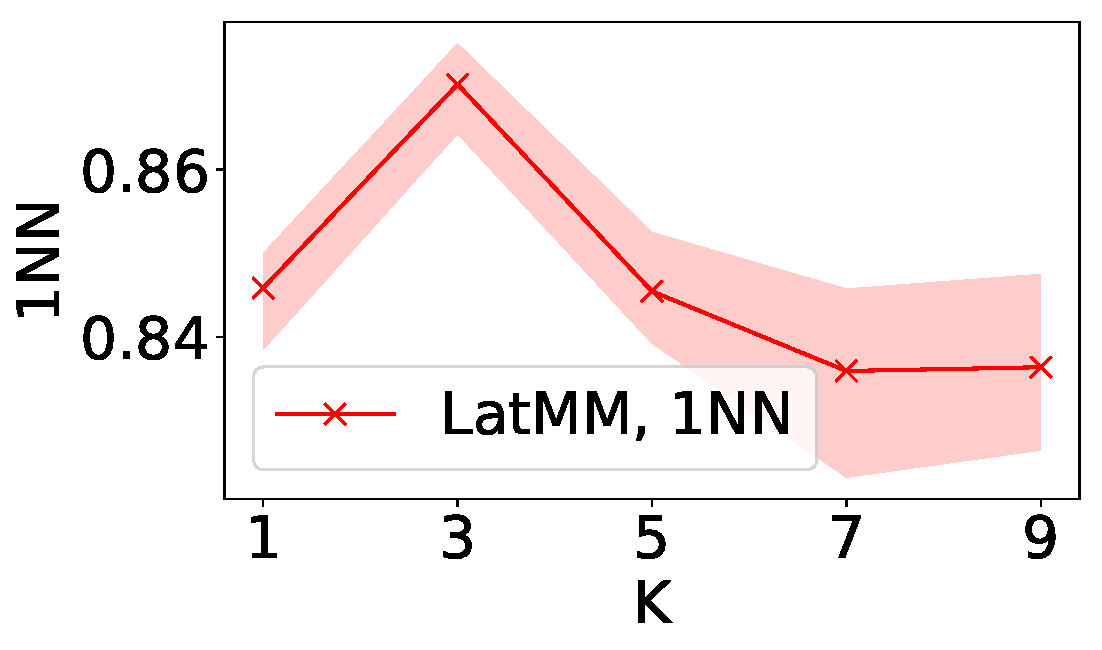
\includegraphics[width=1.\linewidth]{images/fashion-mnist/scores/std1EMGM-SM/EMGM-SM-1NN-K.pdf}
    % \caption{1NN score}
    % \label{fig-sm-1nn}
  \end{subfigure}
  \caption{IS, FID, MMD and 1NN of GenMM and LatMM for
    Fashion-MNIST dataset. GenMM and LatMM are trained on $60000$ images of Fashion-MNIST. The results are evaluated on $2000$ samples
    per simulation point ($1000$ samples generated by GenMM or LatMM
    for corresponding $K$, $1000$ samples from Fashion-MNIST). $5$
    experiments are carried out for each assessed score at each
    setting of $K$. Curve with marker denotes mean score and shaded
    area denotes the range of corresponding
    score.}\label{fig-scores-k-FashionMNIST}
\end{figure*}

\subsection{Evaluation of Proposed Models}
In order to see if the proposed algorithms of GenMM and LatMM help to improve probability distribution modeling capacity, we assess our proposed algorithms with varying number of mixtures ($K$). Since our models are explicit models, the negative log likelihood (NLL) is used for comparison of our models. Apart from NLL, another four different metrics are used in assessment of models.
The metrics are Inception Score (IS) \cite{NIPS2016_6125,2018arXiv180101973B,2018arXiv180607755X}, Frechet
Inception Distance (FID) \cite{2017arXiv170608500H}, Maximum Mean
Discrepancy (MMD) \cite{2018arXiv180607755X} and two-sample test based 1-Nearest
Neighbor (1NN) score \cite{2016arXiv161006545L}. IS measures statistically if a given sample can be recognized by a classifier with high confidence. A high IS stands for high quality for generated samples. FID measures a divergence between two distributions under testing by assuming these two distribution are both Gaussian. We also use MMD with Gaussian kernel to test how dissimilar two distributions are.
Small values of FID and MMD mean that the mixture distribution model
is close to the underlying distribution of dataset. 1NN score measures
if two given distributions are empirically close by computing 1NN accuracy
on samples from two distributions under testing. The closer 1NN score is to $0.5$, the more likely 
two distributions under testing are the same. Therefore, a high IS is good, low FID and MMD scores, and 1NN score close to 0.5 are good. We use the evaluation
framework of \cite{2018arXiv180607755X} to compute these metrics scores, where
we train a ResNet on datasets MNIST and Fashion-MNIST, respectively, as the feature extractor for evaluation of the four performance metrics.



\begin{table}
  \caption{The lowest NLL value of GenMM for curves in Figure~\ref{fig:genmm-nll} (nat/pixel).}
  \label{tab:lowestNLLgenMM}
   \centering
  \begin{tabular}{lcccc}
    \toprule
    {Dataset} & K=1 &  K=3 &  K=5 &  K=7 \\                                         
    \midrule                                                                                          MNIST &     1.8929 &    1.8797 &    1.8719 &    1.8579 \\
    FashionMNIST &   2.3571 &   2.3429 &   2.3353 &   2.3323 \\
    \bottomrule
  \end{tabular} 
\end{table}

The NLL curves of GenMM and LatMM models during model training phase are shown in Figure~\ref{fig:genmm-nll} and Figure~\ref{fig:latmm-nll}, respectively. Subsets of MNIST and Fashion-MNIST are used to train our mixture models in order to assess their performance w.r.t. NLL when different number of mixture components $K$ is used. All the curves in Figure~\ref{fig:genmm-nll} and Figure~\ref{fig:latmm-nll} show that NLL decreases as training epoch number increases in general. There is fluctuation of these decreasing NLL curves due to: (a) the iteration of E-step and M-step of EM, and (b) the use of batch-size gradient in optimization at M-step. In each figure of Figure~\ref{fig:genmm-nll} and Figure~\ref{fig:latmm-nll}, NLL curve corresponding to larger total number of mixture components, $K$, reaches smaller NLL value after traning for same number of epochs. The results are consistent since as $K$ increases, both GenMM and LatMM have smaller NLL. These results confirm our hypothesis that mixture models fit real data better. The lowest NLL values of curves in Figure~\ref{fig:genmm-nll} in training GenMM models are reported in Figure~\ref{tab:lowestNLLgenMM}.

\begin{figure*}[!t]
  \captionsetup[subfigure]{justification=centering}
  \centering
  \begin{subfigure}[b]{0.24\textwidth}
    \centering
    % 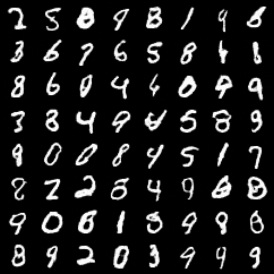
\includegraphics[width=1\linewidth]{images/mnist/samples/gen_c12_std08.png}
    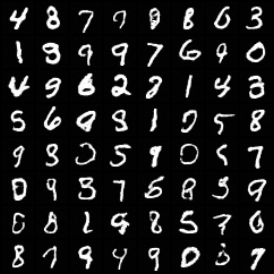
\includegraphics[width=1\linewidth]{images/mnist/samples/genMNIST_GenMM_K7_std089.png}
    \caption{Generated Samples. (GenMM, K=7)}
  \end{subfigure}
  % \begin{subfigure}[b]{0.19\textwidth}
  %   \centering
  %   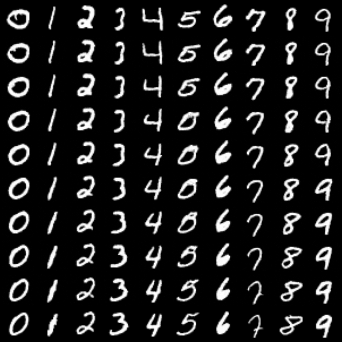
\includegraphics[width=1\linewidth]{images/mnist/interpolation/interpo_c12_mnist_std07.png}
  %   \caption{Interpolation. (GenMM, K=12)}\label{fig-interpo}
  % \end{subfigure}
  \centering
  \begin{subfigure}[b]{0.24\textwidth}
    \centering
    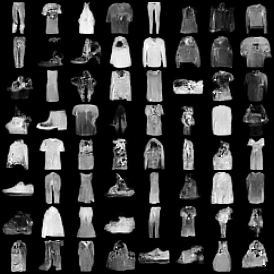
\includegraphics[width=1\linewidth]{images/fashion-mnist/samples/gene_c3_std1_samples.png}
    \caption{Generated samples. (GenMM, K=3)}
  \end{subfigure}
  \begin{subfigure}[b]{0.24\textwidth}
    \centering
    % 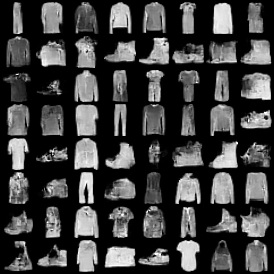
\includegraphics[width=1\linewidth]{images/fashion-mnist/samples/gen_s5_std1.png}
    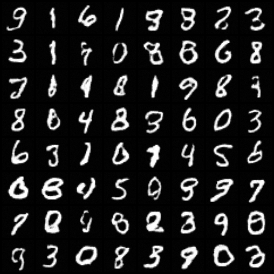
\includegraphics[width=1\linewidth]{images/mnist/samples/gen_LatMM_K3_std088.png}
    \caption{Generated samples. (LatMM, K=3)}
  \end{subfigure}
  \begin{subfigure}[b]{0.24\textwidth}
    \centering
    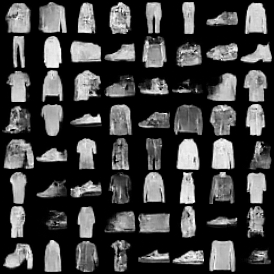
\includegraphics[width=1\linewidth]{images/fashion-mnist/samples/gen_s7_std1.png}
    \caption{Generated samples. (LatMM, K=7)}
  \end{subfigure}
  % \begin{subfigure}[b]{0.23\textwidth}
  %   \centering
  %   \includegraphics[width=1\linewidth]{images/fashion-mnist/samples/gene_c7_std1_samples.png}
  %   \caption{Generated samples. (EMGM-NM, K=7)}
  % \end{subfigure}
  \caption{Generated samples by GenMM and LatMM for MNIST and Fashion-MNIST datasets.}\label{fig-demo-samples}
\end{figure*}
      
\begin{figure*}[!t]
  \centering
  \captionsetup[subfigure]{justification=centering}
  \begin{subfigure}[b]{0.3\textwidth}
    \centering
    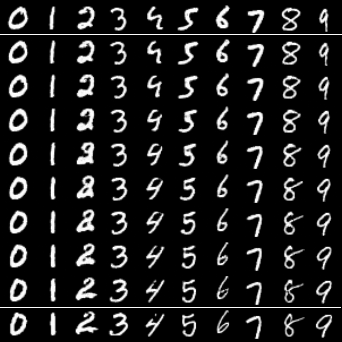
\includegraphics[width=1\linewidth]{images/mnist/interpolation/interpoMNIST_homo_GenMM_K7_map_grid.png}
    \caption{Interpolation by GenMM, K=7. Identity of $\bm{g}_k$ is chosen by $\argmax_{k}\; \gamma_k$.}\label{fig-interpo-genmm1}
  \end{subfigure}
  \hspace{10pt}
  \begin{subfigure}[b]{0.3\textwidth}
    \centering
    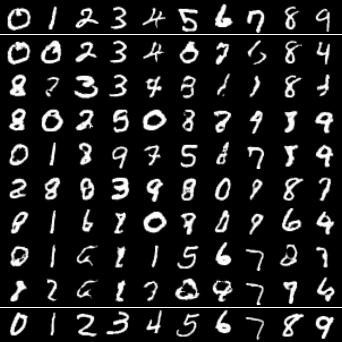
\includegraphics[width=1\linewidth]{images/mnist/interpolation/interpoMNIST_GenMM_K7_random_grid.png}
    \caption{Interpolation by GenMM, K=7. Identity of $\bm{g}_k$ is randomly chosen.~~~~~~~~~}\label{fig-interpo-genmm2}
  \end{subfigure}
  \hspace{10pt}
  \begin{subfigure}[b]{0.3\textwidth}
    \centering
    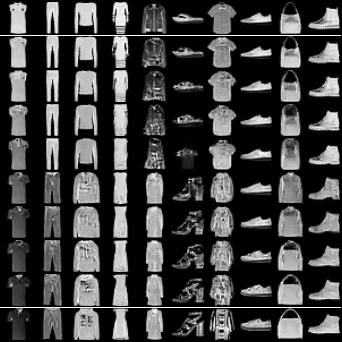
\includegraphics[width=1\linewidth]{images/fashion-mnist/interpolation/interpoFashion_homo_GenMM_K9_map_grid.png}
    \caption{Interpolation by GenMM, K=9. Identity of $\bm{g}_k$ is chosen by $\argmax_{k}\; \gamma_k$.}\label{fig-interpo-genmm3}
  \end{subfigure}
  % \caption{Interpolation in latent space to generate samples . GenMM}\label{fig-interpo}
  \vspace{0.22cm}
  % \label{fig-app-interpolation}
  % \vspace{0.2cm}
  % \end{figure*}
  % \begin{figure*}[!ht]
  \centering
  \captionsetup[subfigure]{justification=centering}
  \begin{subfigure}[b]{0.3\textwidth}
    \centering
    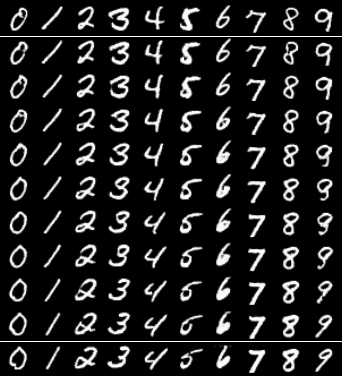
\includegraphics[width=1\linewidth]{images/mnist/interpolation/LatMMK9interpo_sample_grid.png}
    \caption{Interpolation by LatMM, K=9.}\label{fig-interpo-latmm1}
  \end{subfigure}
  \hspace{10pt}
  \begin{subfigure}[b]{0.3\textwidth}
    \centering
    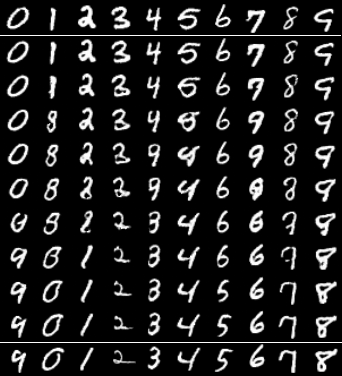
\includegraphics[width=1\linewidth]{images/mnist/interpolation/interpoMNIST_heter_LatMM_K9_sample_grid.png}
    \caption{Interpolation by LatMM, K=9.}\label{fig-interpo-latmm2}
  \end{subfigure}
  \hspace{10pt}
  \begin{subfigure}[b]{0.3\textwidth}
    \centering
    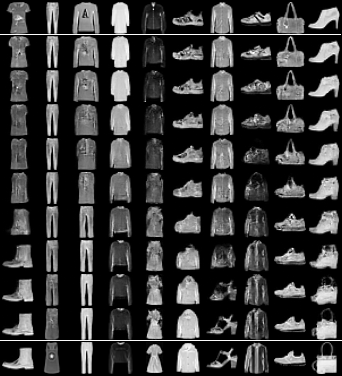
\includegraphics[width=1\linewidth]{images/fashion-mnist/interpolation/interpoFashion_heter_LatMM_K9_grid.png}
    \caption{Interpolation by LatMM, K=9.}\label{fig-interpo-latmm3}
  \end{subfigure}
  \caption{Interpolation in latent space to generate samples . First
    and last rows are real samples from MNIST. For each row, images
    are generated by interpolating latent variables of empirical
    images in first and last rows.}\label{fig-interpo}
  \label{fig-app-interpolation}
\end{figure*}


As for the scores of IS, FID, MMD, and 1NN, we increase $K$ for the proposed models and check
how the four metrics vary. We do several trials of evaluation and
report the results. The results are shown in
Figure~\ref{fig-scores-k} for MNIST datset and
Figure~\ref{fig-scores-k-FashionMNIST} for Fashio-MNIST dataset. Let us
first address the results in Figure~\ref{fig-scores-k}. It can be
observed that IS increases with number of mixtures $K$. The IS
improvement shows a saturation and decreasing trend for GenMM when
$K=9$. The FID, MMD and 1NN scores show a decreasing trend with
increase in $K$. Their trends also saturate with increase in $K$. The
trends obey a statistical knowledge that performance improves with
increase in the model complexity, and then deteriorates if the model
complexity continues to increase. As that in Figure~\ref{fig-scores-k}, similar trends are also observed in Figure~\ref{fig-scores-k-FashionMNIST}. In some cases, performance for $K=3$ is poorer than $K=1$. We assume that the random initialization of parameters in mixture models has a high influence in this regard. 
Considering the trends in all the scores for both the figures, we can conclude that GenMM and LatMM can model the underlying distributions of data and the mixture models are good.

\subsection{Sample Generating and Interpolation}


\begin{figure*}[!ht]
  \captionsetup[subfigure]{justification=centering}
  \centering
  \begin{subfigure}{.31\textwidth}
    \centering
    \includegraphics[width=1\linewidth]{images/supply/train_curves/letter_1.pdf}
    \vspace{-0.8cm}
    \caption{K=1}
    % \label{fig-nm-isk}
  \end{subfigure}
  \begin{subfigure}{.31\textwidth}
    \centering
    \includegraphics[width=1\linewidth]{images/supply/train_curves/letter_2.pdf}
    \vspace{-0.8cm}
    \caption{K=2}
    % \caption{FID score}
    % \label{fig-nm-fidk}
  \end{subfigure}
  \centering
  \begin{subfigure}{.31\textwidth}
    \centering
    \includegraphics[width=1\linewidth]{images/supply/train_curves/letter_3.pdf}
    \vspace{-0.8cm}
    \caption{K=3}
    % \caption{MMD score}
    % \label{fig-nm-mmdk}
  \end{subfigure}
  \centering
  \begin{subfigure}{0.31\textwidth}
    \centering
    \includegraphics[width=1\linewidth]{images/supply/train_curves/letter_4.pdf}
    \vspace{-0.8cm}
    \caption{K=4}
    % \caption{1NN score}
    % \label{fig-nm-1nnk}
  \end{subfigure}
  \centering
  \begin{subfigure}{.31\textwidth}
    \centering
    \includegraphics[width=1\linewidth]{images/supply/train_curves/letter_10.pdf}
    \vspace{-0.8cm}
    \caption{K=10}
    % \caption{IS score}
    % \label{fig-sm-is}
  \end{subfigure}
  \centering
  \begin{subfigure}{.31\textwidth}
    \centering
    \includegraphics[width=1\linewidth]{images/supply/train_curves/letter_20.pdf}
    \vspace{-0.8cm}
    \caption{K=20}
    % \caption{FID score}
    % \label{fig-sm-fid}
  \end{subfigure}
  \caption{Train and Test Accuracy Curves versus Epochs on Dataset Letter.}
  \label{fig:class-letter}
\end{figure*}




Next we show generated samples from the proposed models trained with MNIST and Fashion-MNIST in Figure~\ref{fig-demo-samples}. In the figure, we show generated samples from GenMM and LatMM for MNIST and Fashion-MNIST datasets. We use different value of $K$ to generate images. It can be observed that LatMM is able to produce good quality image samples as GenMM. While we argue that LatMM has a lower level of complexity than GenMM, it is seen that LatMM works good in practice.    

In the second experiment, we explore power of invertibility for interpolation in the latent domain. We use samples from MNIST and Fashion-MNIST datasets for this `interpolation' experiment. In Figure~\ref{fig-interpo}, we have six subfigures. For each subfigure, the first row and the last row are comprised of the real (true) data samples from MNIST and Fashion-MNIST dataset. In each column, we find latent codes corresponding to the real samples of the first row and the last row, $\bm{z}_1, \bm{z}_2$. This is possible as the neural networks are invertible. Then, we perform a convex combination of the two latent codes as $\alpha \bm{z}_1 + (1- \alpha)\bm{z}_2$, where $0 < \alpha <1$. The latent code produced by the convex combination is used to generate a new sample using the trained models. All other rows except the first and the last rows of the figure are the generated samples by varying $\alpha$. In Figure~\ref{fig-interpo}, we observe the change visually from the first row to last row - how the first row slowly changes to the last row. We use GenMM for Figure~\ref{fig-interpo-genmm1}, \ref{fig-interpo-genmm2}, \ref{fig-interpo-genmm3}, and LatMM for Figure~\ref{fig-interpo-latmm1}, \ref{fig-interpo-latmm2}, \ref{fig-interpo-latmm3}. Interpolation experiment for LatMM is easier than GenMM. GenMM has a set of neural network generators $\{ \bm{g}_k(\bm{z}) \}_{k=1}^K$ and a fixed Gaussian distribution for latent variable $\bm{z}$. We compute $\gamma_k$ for a real image $\bm{x}$, and then find the latent code $\bm{z}$ of $\bm{x}$ using $\bm{g}_{k^{*}}^{-1}(\bm{x})=\bm{f}_{k^{*}}(\bm{x})$, where $k^{*} = \arg \max_{k} \gamma_k$. For two real images (one image is in the first row and the second image in the last row), we find the corresponding latent codes, compute their convex combination as interpolation, and then pass the computed latent code through a generator $\bm{g}_k(\bm{z})$ to produce a generated sample $\bm{x}$. Identity of the generator of GenMM is chosen as $k^{*}$ corresponding to the image of the first row if $\alpha < 0.5$, or to the image of the last row if $\alpha \geq 0.5$.

\begin{figure*}[!ht]
  \captionsetup[subfigure]{justification=centering}
  \centering
  \begin{subfigure}{.31\textwidth}
    \centering
    \includegraphics[width=1\linewidth]{images/supply/train_curves/norb_1.pdf}
    \vspace{-0.8cm}
    \caption{K=1}
    % \caption{IS score}
    % \label{fig-nm-isk}
  \end{subfigure}
  \vspace{-2pt}
  \begin{subfigure}{.31\textwidth}
    \centering
    \includegraphics[width=1\linewidth]{images/supply/train_curves/norb_2.pdf}
    \vspace{-0.8cm}
    \caption{K=2}
    % \caption{FID score}
    % \label{fig-nm-fidk}
  \end{subfigure}
  \centering
  \begin{subfigure}{.31\textwidth}
    \centering
    \includegraphics[width=1\linewidth]{images/supply/train_curves/norb_3.pdf}
    \vspace{-0.8cm}
    \caption{K=3}
    % \caption{MMD score}
    % \label{fig-nm-mmdk}
  \end{subfigure}
  \centering
  \begin{subfigure}{0.31\textwidth}
    \centering
    \includegraphics[width=1\linewidth]{images/supply/train_curves/norb_4.pdf}
    \vspace{-0.8cm}
    \caption{K=4}
    % \caption{1NN score}
    % \label{fig-nm-1nnk}
  \end{subfigure}
  \centering
  \begin{subfigure}{.31\textwidth}
    \centering
    \includegraphics[width=1\linewidth]{images/supply/train_curves/norb_10.pdf}
    \vspace{-0.8cm}
    \caption{K=10}
    % \caption{IS score}
    % \label{fig-sm-is}
  \end{subfigure}
  \centering
  \begin{subfigure}{.31\textwidth}
    \centering
    \includegraphics[width=1\linewidth]{images/supply/train_curves/norb_20.pdf}
    \vspace{-0.8cm}
    \caption{K=20}
    % \caption{FID score}
    % \label{fig-sm-fid}
  \end{subfigure}
  \caption{Train and Test Accuracy Curves versus Epochs on Dataset Norb}
  \label{fig:class-norb}
\end{figure*}


The second experiment on interpolation shows interesting result for
modeling multi-modal data. The distribution of ten digits together in
MNIST dataset is expected to be multi-modal. The aspect of multi-modal
distribution is addressed using the experimental result shown in
Figure~\ref{fig-interpo-genmm2}. We use similar experimental steps
as that in Figure~\ref{fig-interpo-genmm1} but with modifications. It
is evident that the generated digit images do not correspond well to
the real images of the first row and the last row. For example, in the
first column of Figure~\ref{fig-interpo-genmm2}, we observe
presence of digits two and eight, while we expect that the
column should be comprised of only images of digit zero. Natural
question is why interpolation leads to generation of digits that are
unexpected. The answer lies in the procedure of performing our
experiment. The key difference for this experiment compared to the
experiment in Figure~\ref{fig-interpo-genmm1} is that a sample is
produced by a randomly selected generator $\bm{g}_k(\bm{z})$ from $K$
possible choices. We compute interpolated latent code using the same
procedure as that in Figure~\ref{fig-interpo-genmm1}, but use the generator where its identity $k$ is randomly sampled from the prior $\bm{\pi}$ directly. The generated images in this interpolation experiment reveals a clue that each generator models a subset of the whole training dataset. We can qualitatively argue that use of multiple generators helps for modeling the multi-modal distribution.  

\subsection{Application to Classification Task}
\begin{table*}[!t]
  \caption{Test Accuracy Table of GenMM for Classification Task}\label{tab:acc-classification}
  % \centering
  % \subcaption{Accuracy Table of GenMM on Test Data}
  % \centering  
  \begin{tabular}{lccccccc} \toprule
    {Dataset} &  K=1 &  K=2 &  K=3 &  K=4 & K=10 & K=20 & State Of Art \\ \midrule
    Letter & 0.9459 &  0.9513 & 0.9578  & 0.9581 & 0.9657 & \textbf{0.9674} & {0.9582} \cite{tang2016extreme} \\ \midrule
    Satimage & 0.8900 & 0.8975 & 0.9045 & 0.9085 & 0.9105 & \textbf{0.9160} & 0.9090 \cite{jiang2013k-svd}   \\ \midrule
    Norb & 0.9184 & 0.9257 & 0.9406 & 0.9459 & 0.9538 & \textbf{0.9542} & 0.8920 \cite{pmlr-v5-salakhutdinov09a}  \\
    \bottomrule
  \end{tabular}
  % \centering
  % \subcaption{Accuracy Table of LatMM}
  % \centering  
  % \begin{tabular}{l|c|c|c|c|c}
      %       \toprule
      %       {Dataset} &  K=1 &  K=2 &  K=3 &  K=4 &  State of Art \\
      %       \midrule
      %       Letter & 0.9453 &  0.9421 &  0.9462 &   0.9469 &  0.9582 \cite{tang2016extreme} \\ \midrule
      %       Satimage & 0.8855 & 0.8895 & 0.8730 & 0.8895 & 0.9090 \cite{jiang2013k-svd} \\ \midrule
      %       Norb & 0.9315 & 0.9221 & 0.9151 & 0.9274 & 0.8920 \cite{pmlr-v5-salakhutdinov09a} \\
      %       \bottomrule                                                                  
      %     \end{tabular}                                                                
\end{table*}

\begin{figure*}[!t]
  \captionsetup[subfigure]{justification=centering}
  \centering
  \begin{subfigure}{.31\textwidth}
    \centering
    \includegraphics[width=1\linewidth]{images/supply/train_curves/satimage_1.pdf}
    \vspace{-0.8cm}
    \caption{K=1}
    % \caption{IS score}
    % \label{fig-nm-isk}
  \end{subfigure}
  \vspace{-2pt}
  \begin{subfigure}{.31\textwidth}
    \centering
    \includegraphics[width=1\linewidth]{images/supply/train_curves/satimage_2.pdf}
    \vspace{-0.8cm}
    \caption{K=2}
    % \caption{FID score}
    % \label{fig-nm-fidk}
  \end{subfigure}
  \centering
  \begin{subfigure}{.31\textwidth}
    \centering
    \includegraphics[width=1\linewidth]{images/supply/train_curves/satimage_3.pdf}
    \vspace{-0.8cm}
    \caption{K=3}
    % \caption{MMD score}
    % \label{fig-nm-mmdk}
  \end{subfigure}
  \centering
  \begin{subfigure}{0.31\textwidth}
    \centering
    \includegraphics[width=1\linewidth]{images/supply/train_curves/satimage_4.pdf}
    \vspace{-0.8cm}
    \caption{K=4}
    % \caption{1NN score}
    % \label{fig-nm-1nnk}
  \end{subfigure}
  \centering
  \begin{subfigure}{.31\textwidth}
    \centering
    \includegraphics[width=1\linewidth]{images/supply/train_curves/satimage_10.pdf}
    \vspace{-0.8cm}
    \caption{K=10}
    % \caption{IS score}
    % \label{fig-sm-is}
  \end{subfigure}
  \centering
  \begin{subfigure}{.31\textwidth}
    \centering
    \includegraphics[width=1\linewidth]{images/supply/train_curves/satimage_20.pdf}
    \vspace{-0.8cm}
    \caption{K=20}
    % \caption{FID score}
    % \label{fig-sm-fid}
  \end{subfigure}
  \caption{Train and Test Accuracy Curves versus Epochs on Dataset Satimage.}
  \label{fig:class-satimage}
\end{figure*}

In this section, we apply our proposed mixture models to classification tasks using the maximum likelihood criterion. We compare classification performance with the state-of-art results. The state-of-art results are produced by discriminative learning approaches. The major advantage of maximum likelihood based classification is that any new class can be accommodated on-the-fly. On the contrary a discriminative learning approach requires retraining whenever new classes appear. 

For a given dataset with $Y$ classes, we divide the dataset by sample labels and each subset has the same label $y$. Then we train one GenMM model per class of data, i.e. $p(\bm{x};\bm{\Theta}_{y})$ is trained with the $y$-th class's data. After we have all $p(\bm{x};\bm{\Theta}_y)$, $\forall y = 1, 2, \cdots, Y$ trained, a new sample $\bm{x}$ is predicted by $\argmax_{y} p(\bm{x};\bm{\Theta}_y)$.

The maximum likelihood based classification experiment as described above is carried out in three different datasets: Letter, Satimage, and Norb. For each dataset, we train our models for $300$ epoches on the training data of the corresponding dataset, and the test accuracy is reported in Table~\ref{tab:acc-classification}. The state-of-art accuracy of each dataset in literature is also listed in this table for comparison. For each dataset, we increase the total number of mixture components $K$ and the neural network generators have the same structure. The table shows that the classification accuracy on each dataset is increased as we increase the number of generators in GenMM. When $K$ is $10$ or $20$, maximum likelihood based classification by GenMM outperforms the state-of-art accuracy. The state-of-art accuracy results are obtained by using discriminative learning approaches. For dataset Norb, more significant performance gain is observed. Our classification accuracy is boosted from $0.9184$ to $0.9542$ when $K$ is increased from $1$ to $20$ and a large improvement margin is obtained over reference accuracy. We also test LatMM on classification task, but its accuracy is more or less around the accuracy of GenMM with $K=1$. Note that LatMM is a relatively low-complexity model than GenMM. 

Figure~\ref{fig:class-letter}, \ref{fig:class-satimage} and \ref{fig:class-norb} show the train and test accuracy changing along with the training epoch on dataset Letter and Satimage, respectively. For each dataset, the accuracy curves versus epoch trained with GenMM at different value of $K$ are shown. In these sets of figures, all accuracy curves climbs and flattens around some value, as training epoch increases. Train accuracy is either coincident with, or above test accuracy curve at different training phases. For each set of figures on a given dataset, the gap between train and test curve is smaller as a larger number of mixture components is used. As $K$ increases, test curve flattens at a larger accuracy value. This again speaks for validation of our proposed models and also the advantage of using our mixture models for practical tasks.

\section{Summary}
In this chapter, we considered the learning problem in the presence of incomplete data (or unobserved variables) in directed graphs. We introduced normalizing flows that ware implemented as neural networks to model the conditional distributions, in order to increase modeling flexibility. Building a model more expressively helps reduces the inherent bias in modeling. The proposed models allow both exact likelihood computation and also efficient sampling.

Learning methods of the proposed models ware proposed. Due to the presence of neural network based flows in conditional distribution modeling, expectation maximization was tailored to adapt to their learning and the maximization step was approximately solved with back-propagation technique. The approximation was also partially due to the fact that batch-based optimization had to been used to accommodate large datasets. From the perspective of the numerical evaluations, the proposed models are valid. The numerical results show that the normal statistical behavior of modeling performance versus model complexity remains valid. More expressive models benefit the applications to data representation (data generating) and classification.

The considered models in this chapter assume that an observation instance with its unobserved variable is independent of other observation instances (with their corresponding hidden variables). This assumption could bring poor models when the true signal is temporal and the independence does not hold. In the next chapter, we would consider how to model and learn a model where this independence is gone. 

\section{Related Work}

Using mixture models to get gain in modeling flexibility is a typical technique, which is especially useful when the target dataset is multi-modal. This gain comes with unobserved variables. The unobserved variables usually are related to the abstraction of data modal, which helps us interpret the data. But they also pose challenges in model learning. In literature, expectation maximization \cite{dempster1977maximum} is a standard approach for learning parameters of an explicit mixture model where the likelihood is tractable. Gaussian mixture model is the most classic one in this framework \cite{Bishop:2006:PRM:1162264}.
Apart from explicit likelihood, when sufficient statistics are explicitly present in a model, stochastic EM \cite{cappe2009sem} is applicable to accommodate large datasets. Instead of computing expectation step w.r.t. every datum, stochastic EM carries out expectation step w.r.t. a randomly selected datum to reduce the complexity of vanilla EM. The benefit of reduced complexity comes with the drawback of increased variance in parameter learning. This issue triggered the stochastic EM with variance reduction\cite{chen2018emvr} and fast incremental EM \cite{karimi2019incrementalEM} methods.


When likelihood is not tractable (e.g., implicit probabilistic models), different objectives need to be designed to guide the modeling learning. Generative adversarial networks (GANs) have gained increasing attention in this track \cite{NIPS2014_5423, NIPS2016_6125, 2018arXiv180508318Z, salimans2018improving}.
GANs are efficient for generating samples and successful in several applications \cite{ledig2017photo, NIPS2016_6125}. In a GAN, a latent variable is used as
an input to the generator neural network of the GAN, and the output of the neural network is considered to be a data sample from an implicit distribution. The implicit distraction targets at approximating the underlying distribution of the given dataset, via the guidance of a discriminator.
To capture diversity in data (multi-modal), the usage of multiple generators has been considered. For instance, multiple Wasserstein GANs \cite{2017arXiv170107875A} are used in \cite{2018arXiv180600880K} with appropriate mutual information based regularization to encourage the diversity of samples generated by different GANs.
A mixture GAN approach is proposed in \cite{hoang2018mgan} using multiple generators and multi-classification solution to
encourage diversity of samples. Multi-agent diverse GAN \cite{DBLP:journals/corr/GhoshKNTD17} similarly employs $k$ generators, but uses a $(k+1)$-class discriminator instead of a typical binary discriminator to increase the diversity of generated samples. These works are implicit probability distribution modeling and thus empirical or appropriate methods have to been used to cope with the unobserved random variable. For instance, extra neural networks are used to model the posterior of the unobserved variables \cite{donahue2017adversarial, dumoulin2017adversarially}. 


Another track of mixture modeling is based on the ensembling method that combines weaker learners together to boost the overall performance \cite{grover2017aaai_boost,2017arXiv170102386T}. In this approach, mixture models are obtained as follows. Based on how well the current-step mixture model captures the underlying distribution, a new generative model is trained to compensate for the miss-captured part. However, measuring the difference between the current-step mixture model and the underlying distribution of the dataset quantitatively is a nontrivial task, especially when the likelihood is not tractable. In addition, since incremental building components are used in the mixture modeling, parallel training of model components is not allowed.






%%% Local Variables:
%%% mode: latex
%%% TeX-master: "../../main"
%%% End:
